\chapter{多元函数微分法}
在前面章节中讨论的函数是一元函数,它只有一个实自变量和一个实因变量.
但在实际问题中,可能会有多方面的因素影响,也就是说我们需要进一步研究二元函数、多元函数和向量值函数.

\section{多元函数的极限}
\subsection{重极限的概念}
\begin{definition}
设二元函数\(f(P)=f(x,y)\)的定义域为\(D\),\(P_0(x_0,y_0)\)是\(D\)的聚点.
如果存在常数\(A\),对于\(\forall \varepsilon > 0\),\(\exists \delta > 0\),
使得当\(P(x,y) \in D \cap \mathring{U}(P_0,\delta)\)时,都有\[
	\abs{f(P)-A} = \abs{f(x,y)-A} < \varepsilon
\]成立,
那么称常数\(A\)为“函数\(f(x,y)\)当\((x,y)\to(x_0,y_0)\)时的\DefineConcept{极限}”,记作\[
	\lim\limits_{(x,y)\to(x_0,y_0)} f(x,y) = A
	\quad\text{或}\quad
	\lim\limits_{P \to P_0} f(P) = A.
\]

为了区别于一元函数的极限,我们把二元函数的极限叫做\DefineConcept{二重极限}.
\end{definition}

\begin{example}
设\(f(x,y) = (x^2+y^2) \sin\frac{1}{x^2+y^2}\),求证:\(\lim\limits_{(x,y)\to(0,0)} f(x,y) = 0\).
\begin{solution}
这里函数\(f(x,y)\)的定义域为\(D = \mathbb{R}^2 - \Set{(0,0)}\),点\(O(0,0)\)为\(D\)的聚点.因为\[
\abs{f(x,y)-0}
= \abs{(x^2+y^2) \sin\frac{1}{x^2+y^2} - 0}
\leq x^2+y^2,
\]可见,\(\forall\varepsilon>0\),取\(\delta=\sqrt{\varepsilon}\),则当\[
0 < \sqrt{(x-0)^2+(y-0)^2} < \delta,
\]即\(P(x,y) \in D \cap \mathring{U}(O,\delta)\)时,总有\[
\abs{f(x,y)-0} < \varepsilon
\]成立,所以\[
\lim\limits_{(x,y)\to(0,0)} f(x,y) = 0.
\]
\end{solution}
\end{example}

必须注意,所谓二重极限存在,
是指\(P(x,y)\)以任何方式趋于\(P_0(x_0,y_0)\)时,\(f(x,y)\)都无限接近于\(A\).
因此,如果\(P(x,y)\)以某一特殊方式,
例如沿着一条定直线或定曲线趋于\(P_0(x_0,y_0)\)时,
即使\(f(x,y)\)无限接近于某一确定值,
我们还不能由此断定函数的极限存在.
但是反过来,如果当\(P(x,y)\)以不同方式趋于\(P_0(x_0,y_0)\)时,
\(f(x,y)\)趋于不同的值,那么就可以断定这函数的极限不存在.

以上关于二元函数的极限概念,可相应地推广到\(n\)元函数\(u = f(P)\),
即\(u = f(\AutoTuple{x}{n})\)上去.
\begin{definition}
设\(n\)元函数\(f(\mat{x})\)的定义域为\(D \subseteq \mathbb{R}^n\),点\(\mat{a}\)是\(D\)的聚点.
如果存在常数\(A \in \mathbb{R}\),
对于\(\forall\varepsilon>0\),
\(\exists\delta>0\),
使得当\(\mat{x} \in D \cap \mathring{U}(\mat{a},\delta)\)时,
都有\[
	\abs{f(\mat{x}) - A} < \varepsilon
\]成立,
则称常数\(A\)为“函数\(f(\mat{x})\)当\(\mat{x}\to\mat{a}\)时的\DefineConcept{极限}”,记作\[
	\lim\limits_{\mat{x}\to\mat{a}} f(\mat{x}) = A.
\]
\end{definition}

多元函数的极限遵从与一元函数类似的性质与极限运算法则,
例如\hyperref[theorem:极限.函数极限的唯一性]{唯一性}、
\hyperref[theorem:极限.函数极限的局部有界性]{局部有界性}、
\hyperref[theorem:极限.函数极限的局部保号性1]{局部保号性}、
\hyperref[theorem:极限.海涅定理]{海涅定理}、
\hyperref[theorem:极限.夹逼准则]{夹逼准则}、
\hyperref[theorem:极限.极限的四则运算法则]{四则运算法则}.

\begin{example}
\def\l{\lim\limits_{\opair{x,y}\to\opair{0,2}}}
求\(\l \frac{\sin(xy)}{x}\).
\begin{solution}
函数\(\frac{\sin(xy)}{x}\)的定义域为\[
D = \Set{ \opair{x,y} \given x\neq0, y\in\mathbb{R} },
\]点\(P_0\opair{0,2}\)为\(D\)的聚点.

由积的极限运算法则,得\[
\l \frac{\sin(xy)}{x}
= \l \left[ \frac{\sin(xy)}{xy} \cdot y \right]
= \lim\limits_{xy\to0} \frac{\sin(xy)}{xy} \cdot \lim\limits_{y\to2} y
= 1 \cdot 2 = 2.
\]
\end{solution}
\end{example}

\subsection{累次极限的概念}
\begin{definition}
设二元函数\(f(x,y)\)的定义域是\(D = D_1 \times D_2 \subseteq \mathbb{R}^2\),点\(x_0\)、\(y_0\)分别是\(D_1\)、\(D_2\)的聚点.
如果对\(\forall y_1 \in D_2 - \{y_0\}\),关于\(x\)的一元函数\(f(x,y_1)\)的极限\[
\lim\limits_{\substack{x \to x_0 \\ (x \in D_1)}} f(x,y_1)
\]存在,且极限\[
\lim\limits_{\substack{y \to y_0 \\ (y \in D_2)}} \lim\limits_{\substack{x \to x_0 \\ (x \in D_1)}} f(x,y)
\]也存在,则称后者为\(f(x,y)\)在点\((x_0,y_0)\)先\(x\)后\(y\)的\DefineConcept{累次极限}(repeated limit),简记为\[
\lim\limits_{y \to y_0} \lim\limits_{x \to x_0} f(x,y).
\]

类似地,可以定义先\(y\)后\(x\)的累次极限\[
\lim\limits_{x \to x_0} \lim\limits_{y \to y_0} f(x,y).
\]
\end{definition}

\begin{example}
重极限和累次极限的关系是很复杂的.
\begin{enumerate}
\item 有时候,重极限存在,但两个累次极限都不存在.比如\[
f(x,y) = \left\{ \begin{array}{cl}
x \sin(1/y) + y \sin(1/x), & x\neq0 \land y\neq0, \\
0, & x=0 \lor y=0.
\end{array} \right.
\]的重极限\[
\lim\limits_{\opair{x,y}\to(0,0)} f(x,y) = 0.
\]

\item 有时候,重极限存在,但两个累次极限中一个存在而另一个不存在.比如\[
g(x,y) = \left\{ \begin{array}{cl}
x \sin(1/y), & y\neq0, \\
0, & y=0.
\end{array} \right.
\]的重极限\[
\lim\limits_{\opair{x,y}\to(0,0)} g(x,y) = 0;
\]又有\[
\lim\limits_{y\to0} \lim\limits_{x\to0} g(x,y) = 0,
\]而\[
\lim\limits_{x\to0} \lim\limits_{y\to0} g(x,y)
\]不存在.

\item 有时候,两个累次极限都存在且相等,但重极限不存在.比如\[
h(x,y) = \left\{ \begin{array}{cl}
\frac{xy}{x^2+y^2}, & \opair{x,y}\neq(0,0), \\
0, & \opair{x,y}=(0,0).
\end{array} \right.
\]的重极限不存在;而\[
\lim\limits_{x\to0} \lim\limits_{y\to0} h(x,y)
= \lim\limits_{y\to0} \lim\limits_{x\to0} h(x,y) = 0.
\]

\item 有时候,两个累次极限都存在,但不相等.比如\[
\varphi(x,y) = \frac{x^2(1+x^2) - y^2(1+y^2)}{x^2+y^2}
\]的两个累次极限分别为\[
\lim\limits_{x\to0} \lim\limits_{y\to0} \varphi(x,y) = 1,
\qquad
\lim\limits_{y\to0} \lim\limits_{x\to0} \varphi(x,y) = -1.
\]
\end{enumerate}
\end{example}

\begin{theorem}
设二元函数\(f(x,y)\)在点\((x_0,y_0)\)处存在重极限\[
\lim\limits_{\opair{x,y}\to(x_0,y_0)} f(x,y) = A \in \mathbb{R}.
\]\begin{enumerate}
\item 如果当\(y \neq y_0\)时存在极限\[
\lim\limits_{x \to x_0} f(x,y) = \psi(y),
\]则\(f(x,y)\)在点\((x_0,y_0)\)处的先\(x\)后\(y\)的累次极限存在,且\[
\lim\limits_{y \to y_0} \lim\limits_{x \to x_0} f(x,y)
= \lim\limits_{y \to y_0} \psi(y) = A.
\]

\item 如果当\(x \neq x_0\)时存在极限\[
\lim\limits_{y \to y_0} f(x,y) = \varphi(y),
\]则\(f(x,y)\)在点\((x_0,y_0)\)处的先\(y\)后\(x\)的累次极限存在,且\[
\lim\limits_{x \to x_0} \lim\limits_{y \to y_0} f(x,y)
= \lim\limits_{x \to x_0} \varphi(y) = A.
\]
\end{enumerate}
\end{theorem}

\begin{corollary}
如果两个累次极限和重极限都存在,则三者必定相等.
\end{corollary}

\begin{corollary}
如果两个累次极限都存在但不相等,则重极限必定不存在.
\end{corollary}

\section{多元函数的连续性}
\begin{definition}
设二元函数\(f(P)=f(x,y)\)的定义域为\(D\),\(P_0(x_0,y_0)\)是\(D\)的聚点,且\(P_0 \in D\).如果\[
\lim\limits_{\opair{x,y}\to(x_0,y_0)} f(x,y) = f(x_0,y_0),
\]则称“函数\(f(x,y)\)在点\(P_0(x_0,y_0)\) \DefineConcept{连续}”.

设二元函数\(f(x,y)\)在\(D\)上有定义,\(D\)内的每一点都是函数定义域的聚点.
如果函数\(f(x,y)\)在\(D\)的每一点都连续,那么称函数\(f(x,y)\)在\(D\)上连续,或者称\(f(x,y)\)是\(D\)上的\DefineConcept{连续函数}.
\end{definition}
以上关于二元函数的连续性概念,可相应地推广到\(n\)元函数\(f(P)\)上去.

一元初等函数\(f(x)\)看成二元函数或二元以上的多元函数\(F(x,y_1,y_2,\dotsc,y_n)\)时,即\[
F(x,y_1,y_2,\dotsc,y_n) = f(x),
\]总有\(F(x,y_1,y_2,\dotsc,y_n)\)在各自的定义域内都是连续的.

\begin{definition}
设函数\(f(x,y)\)的定义域为\(D\),\(P_0(x_0,y_0)\)是\(D\)的聚点.
如果函数\(f(x,y)\)在点\(P_0(x_0,y_0)\)不连续,则称\(P_0(x_0,y_0)\)为函数\(f(x,y)\)的\DefineConcept{间断点}.
\end{definition}

前面已经指出:一元函数中关于极限的运算法则,对于多元函数仍然适用.
根据多元函数的极限运算法则,可以证明多元连续函数的和、差、积仍为连续函数;
连续函数的商在分母不为零处仍连续;
多元连续函数的复合函数也是连续函数.

与一元初等函数相类似,\DefineConcept{多元初等函数}是指可用一个式子表示的多元函数,这个式子是由常数及具有不同自变量的一元基本初等函数经过有限次的四则运算和复合运算而得到的.
例如\(\frac{x+x^2-y^2}{1+y^2},\sin(x+y),\exp(x^2+y^2+z^2)\)等都是多元初等函数.

根据上面指出的连续函数的和、差、积、商的连续性以及连续函数的复合函数的连续性,再利用基本初等函数的连续性,我们进一步可以得出如下揭露:

一切多元初等函数在其定义区域内是连续的.
所谓定义区域是指包含于定义域内的开区域或闭区域.

由多元初等函数的连续性,如果要求它在点\(P_0\)处的极限,而该点又在此函数的定义区域内,则极限值就是函数在该点的函数值,即\[
\lim\limits_{P \to P_0} f(P) = f(P_0).
\]

\begin{example}
\def\l{\lim\limits_{\opair{x,y}\to(0,0)}}
求\(\l \frac{\sqrt{xy+1}-1}{xy}\).
\begin{solution}
\[\begin{split}
\l \frac{\sqrt{xy+1}-1}{xy}
&= \l \frac{xy+1-1}{xy(\sqrt{xy+1}+1)} \\
&= \l \frac{1}{\sqrt{xy+1}+1}
= \frac{1}{2}.
\end{split}\]
\end{solution}
\end{example}

与闭区间上一元连续函数的性质相类似,在有界闭区域上连续的多元函数具有如下性质.

\begin{property}[有界性与最值定理]\label{theorem:多元函数微分法.有界性与最值定理}
在有界闭区域\(D\)上的多元连续函数,必定在\(D\)上有界,且能取得它的最大值和最小值.
\end{property}

\begin{property}[介值定理]\label{theorem:多元函数微分法.介值定理}
在有界闭区域\(D\)上的多元连续函数必取得介于最大值和最小值之间的任何值.
\end{property}

\begin{property}[一致连续性定理]\label{theorem:多元函数微分法.一致连续性定理}
在有界闭区域\(D\)上的多元连续函数必定在\(D\)上\DefineConcept{一致连续}.

也就是说,若多元连续函数\(f(P)\)在有界闭区域\(D\)上连续,则对于\(\forall \varepsilon > 0\),\(\exists \delta > 0\),使得对于\(\forall P_1,P_2 \in D\),只要当\(\abs{P_1P_2}<\delta\)时,都有\[
\abs{f(P_1)-f(P_2)} < \varepsilon
\]成立.
\end{property}

\section{偏导数}
\subsection{偏导数的定义及其计算法}
\subsubsection{偏导数的概念}
\begin{definition}
设函数\(z=f(x,y)\)在点\((x_0,y_0)\)的某一邻域内有定义,
当\(y\)固定在\(y_0\)而\(x\)在\(x_0\)处有增量\(\increment x\)时,
相应的函数有增量\[
	f(x_0+\increment x,y_0)-f(x_0,y_0).
\]
如果\[
	\lim\limits_{\increment x\to0}
	\frac{f(x_0+\increment x,y_0)-f(x_0,y_0)}{\increment x}
\]存在,
则称此极限为
“函数\(z=f(x,y)\)
在点\((x_0,y_0)\)处
对\(x\)的\DefineConcept{偏导数}(partial derivative)”,记作\[
	\eval{\pdv{z}{x}}_{\substack{x=x_0 \\ y=y_0}},\quad
	\eval{\pdv{f}{x}}_{\substack{x=x_0 \\ y=y_0}},\quad
	\eval{z'_x}_{\substack{x=x_0 \\ y=y_0}}
	\quad\text{或}\quad
	f'_x(x_0,y_0).
\]

类似地,可以定义函数\(z=f(x,y)\)在点\((x_0,y_0)\)处对\(y\)的偏导数\[
\lim\limits_{\increment y\to0} \frac{f(x_0,y_0+\increment y)-f(x_0,y_0)}{\increment y},
\]记作\[
\eval{\pdv{z}{y}}_{\substack{x=x_0 \\ y=y_0}},\quad
\eval{\pdv{f}{y}}_{\substack{x=x_0 \\ y=y_0}},\quad
\eval{z'_y}_{\substack{x=x_0 \\ y=y_0}} \quad
\text{或}\quad
f'_y(x_0,y_0).
\]

如果函数\(z=f(x,y)\)在区域\(D\)内每一点\(\opair{x,y}\)处对\(x\)的偏导数都存在,那么这个偏导数就是\(x\)、\(y\)的函数,它就称为函数\(z=f(x,y)\)对自变量\(x\)的\DefineConcept{偏导函数},记作\[
\pdv{z}{x},\quad
\pdv{f}{x},\quad
z'_x \quad
\text{或}\quad
f'_x(x,y).
\]

类似地,可以定义函数\(z=f(x,y)\)对自变量\(y\)的偏导函数,记作\[
\pdv{z}{y},\quad
\pdv{f}{y},\quad
z'_y \quad
\text{或}\quad
f'_y(x,y).
\]
\end{definition}

偏导数的概念还可以推广到二元以上的函数.
\begin{definition}
设\(n\)元函数\(y=f(\AutoTuple{x}{n})\)在点\(P\opair{\AutoTuple{a}{n}}\)的某一邻域内有定义.
如果极限\[
\lim\limits_{\increment x_k\to0}
 \frac{f(a_1,\dotsc,a_k+\increment x_k,\dotsc,a_n) - f(a_1,\dotsc,a_k,\dotsc,a_n)}{\increment x_k}
 \quad (k=1,2,\dotsc,n)
\]存在,则称此极限为函数\(f\)在点\(P\)处对\(x_k\)的偏导数,记作\[
\eval{\pdv{f}{x_k}}_{\mat{x}=\mat{a}}
\quad\text{或}\quad
f'_{x_k}(\AutoTuple{a}{n}).
\]

如果函数\(f\)在点\(P\)的某个邻域内每一点处对\(x_k\)的偏导数都存在,且这个偏导函数\[
f'_{x_k}(\AutoTuple{x}{n})
\]在点\(P\)连续,那么称这个偏导数\DefineConcept{连续}.
\end{definition}

可以证明,在计算任意二元函数\(f(x,y)\)在点\((x_0,y_0)\)处的偏导数(以\(\eval{\pdv{f}{x}}_{(x_0,y_0)}\)为例)时,可以先将不变量\(y_0\)代入,将问题转化为计算一元函数\(z = f(x, y_0)\)的导数\(\eval{\dv{z}{x}}_{x=x_0}\).

\begin{example}
已知理想气体的状态方程\[
pV = RT,
\]其中\(R\)为常量,求证:\[
\pdv{p}{V} \cdot \pdv{V}{T} \cdot \pdv{T}{p} = -1.
\]
\begin{proof}
因为\[
p = \frac{RT}{V}, \qquad \pdv{p}{V} = -\frac{RT}{V^2};
\]\[
V = \frac{RT}{p}, \qquad \pdv{V}{T} = \frac{R}{p};
\]\[
T = \frac{pV}{R}, \qquad \pdv{T}{p} = \frac{V}{R};
\]所以\[
\pdv{p}{V} \cdot \pdv{V}{T} \cdot \pdv{T}{p}
= -\frac{RT}{V^2} \cdot \frac{R}{p} \cdot \frac{V}{R}
= -\frac{RT}{pV} = -1.
\qedhere
\]
\end{proof}
\end{example}

我们知道,对一元函数来说,\(\dv{y}{x}\)可看做函数的微分\(\dd{y}\)与自变量的微分\(\dd{x}\)之商.
而上例表明,偏导数的记号是一个整体记号,不能看作分子与分母之商.

\subsubsection{偏导数的几何意义}
二元函数\(z=f(x,y)\)在点\((x_0,y_0)\)的偏导数有下述几何意义.
偏导数\(f'_x(x_0,y_0)\)的几何意义是曲面\(z=f(x,y)\)被平面\(y=y_0\)所截得的曲线在点\(M_0\opair{x_0,y_0,f(x_0,y_0)}\)处的切线对\(x\)轴的斜率.

\subsubsection{偏导数与连续性的关系}
我们已经知道,如果一元函数在某点具有导数,则它在该点必定连续.
但对于多元函数来说,即使各偏导数在某点都存在,也不能保证函数在该点连续.
这是因为各偏导数存在只能保证点\(P\)沿着平行于坐标轴的方向趋于\(P_0\)时,函数值\(f(P)\)趋于\(f(P_0)\),但不能保证点\(P\)按任何方式趋于\(P_0\)时,函数值\(f(P)\)都趋于\(f(P_0)\).

\subsection{高阶偏导数}
\begin{definition}
设函数\(z=f(x,y)\)在区域\(D\)内具有偏导数\[
\pdv{z}{x} = f_x(x,y), \qquad
\pdv{z}{y} = f_y(x,y).
\]如果\(f'_x(x,y)\)和\(f'_y(x,y)\)在区域\(D\)内的偏导数也存在,则称它们是函数\(z=f(x,y)\)的\DefineConcept{二阶偏导数}.
按照对变量求导次序的不同有下列四个二阶偏导数:
\begin{gather*}
\pdv{x}(\pdv{z}{x}) = \pdv[2]{z}{x} = f''_{xx}(x,y),
\qquad
\pdv{y}(\pdv{z}{x}) = \pdv{z}{x}{y} = f''_{xy}(x,y), \\
\pdv{x}(\pdv{z}{y}) = \pdv{z}{y}{x} = f''_{yx}(x,y),
\qquad
\pdv{y}(\pdv{z}{y}) = \pdv[2]{z}{y} = f''_{yy}(x,y),
\end{gather*}
其中\(f''_{xy}(x,y)\)和\(f''_{yx}(x,y)\)称为\DefineConcept{混合偏导数}.
二阶及二阶以上的偏导数统称为\DefineConcept{高阶偏导数}.
\end{definition}

\begin{theorem}
如果函数\(z=f(x,y)\)的两个二阶混合偏导数\(\pdv{z}{y}{x}\)及\(\pdv{z}{x}{y}\)在区域\(D\)内连续,
那么在该区域内这两个二阶混合偏导数必相等.
\begin{proof}
根据偏导数的定义,我们有
\[
	\pdv{z(x,y)}{x}
	= \lim\limits_{\increment x\to0} \frac{f(x+\increment x,y)-f(x,y)}{\increment x},
\]
	\[
	\pdv{z(x,y)}{y}
	= \lim\limits_{\increment y\to0} \frac{f(x,y+\increment y)-f(x,y)}{\increment y}.
\]
于是,我们就有
\begin{align*}
	\pdv[2]{z}{x}{y}
	&= \lim\limits_{\increment y\to0}
		\frac{1}{\increment y}\left[\pdv{z(x,y+\increment y)}{x} - \pdv{z(x,y)}{x}\right] \\
	&= \lim\limits_{\increment y\to0}
		\frac{1}{\increment y}\left[\lim\limits_{\increment x\to0} \frac{f(x+\increment x,y+\increment y)-f(x,y+\increment y)}{\increment x} - \lim\limits_{\increment x\to0} \frac{f(x+\increment x,y)-f(x,y)}{\increment x}\right] \\
	&= \lim\limits_{\increment y\to0}
		\frac{1}{\increment y}\left\{\lim\limits_{\increment x\to0} \frac{[f(x+\increment x,y+\increment y)-f(x,y+\increment y)]-[f(x+\increment x,y)-f(x,y)]}{\increment x}\right\} \\
	&= \lim\limits_{\increment y\to0} \lim\limits_{\increment x\to0}
		\frac{f(x+\increment x,y+\increment y)-f(x,y+\increment y)-f(x+\increment x,y)+f(x,y)}{\increment x \cdot \increment y}, \\
	\pdv[2]{z}{y}{x}
	&= \lim\limits_{\increment x\to0}
		\frac{1}{\increment x}\left[\pdv{z(x+\increment x,y)}{y} - \pdv{z(x,y)}{y}\right] \\
	&= \lim\limits_{\increment x\to0}
		\frac{1}{\increment x}\left[\lim\limits_{\increment y\to0} \frac{f(x+\increment x,y+\increment y)-f(x+\increment x,y)}{\increment y} - \lim\limits_{\increment y\to0} \frac{f(x,y+\increment y)-f(x,y)}{\increment y}\right] \\
	&= \lim\limits_{\increment x\to0}
		\frac{1}{\increment x}\left\{\lim\limits_{\increment y\to0} \frac{[f(x+\increment x,y+\increment y)-f(x+\increment x,y)]-[f(x,y+\increment y)-f(x,y)]}{\increment y}\right\} \\
	&= \lim\limits_{\increment x\to0} \lim\limits_{\increment y\to0}
		\frac{f(x+\increment x,y+\increment y)-f(x+\increment x,y)-f(x,y+\increment y)+f(x,y)}{\increment x \cdot \increment y}, \\
\end{align*}
显然\[
	\pdv[2]{z}{x}{y} = \pdv[2]{z}{y}{x}.
	\qedhere
\]
\end{proof}
\end{theorem}
换句话说,二阶混合偏导数在连续的条件下与求导的次序无关.
同样地,高阶混合偏导数在连续的条件下也与求导的次序无关.

\begin{example}
验证函数\(z = \ln\sqrt{x^2+y^2}\)满足方程\[
\pdv[2]{z}{x} + \pdv[2]{z}{y} = 0.
\]
\begin{proof}
因为\(z = \ln\sqrt{x^2+y^2} = \frac{1}{2} \ln(x^2+y^2)\),所以\[
\pdv{z}{x} = \frac{x}{x^2+y^2},
\qquad
\pdv{z}{y} = \frac{y}{x^2+y^2},
\]\[
\pdv[2]{z}{x} = \frac{(x^2+y^2)-x\cdot2x}{(x^2+y^2)^2}
= \frac{y^2-x^2}{(x^2+y^2)^2},
\]\[
\pdv[2]{z}{y} = \frac{(x^2+y^2)-y\cdot2y}{(x^2+y^2)^2}
= \frac{x^2-y^2}{(x^2+y^2)^2},
\]因此\[
\pdv[2]{z}{x} + \pdv[2]{z}{y}
= \frac{y^2-x^2}{(x^2+y^2)^2} + \frac{x^2-y^2}{(x^2+y^2)^2}
= 0.
\qedhere
\]
\end{proof}
\end{example}

\begin{example}
证明函数\(u = \frac{1}{r}\)满足方程\[
\pdv[2]{u}{x} + \pdv[2]{u}{y} + \pdv[2]{u}{z} = 0,
\]其中\(r = \sqrt{x^2+y^2+z^2}\).
\begin{proof}
显然有\[
\pdv{u}{x} = -\frac{1}{r^2}\cdot\pdv{r}{x}
= -\frac{1}{r^2}\cdot\frac{x}{r}
= -\frac{x}{r^3},
\]\[
\pdv[2]{u}{x} = -\frac{1}{r^3} + \frac{3x}{r^4}\cdot\pdv{r}{x}
= -\frac{1}{r^3} + \frac{3x^2}{r^5}.
\]由于函数关于自变量的对称性,所以\[
\pdv[2]{u}{y} = -\frac{1}{r^3} + \frac{3y^2}{r^5},
\qquad
\pdv[2]{u}{z} = -\frac{1}{r^3} + \frac{3z^2}{r^5},
\]因此\[
\pdv[2]{u}{x} + \pdv[2]{u}{y} + \pdv[2]{u}{z}
= -\frac{3}{r^3} + 3\frac{x^2+y^2+z^2}{r^5}
= -\frac{3}{r^3} + 3\frac{r^2}{r^5} = 0.
\qedhere
\]
\end{proof}
\end{example}

\begin{example}
验证函数\(r = \sqrt{x^2+y^2+z^2}\)满足\[
\pdv[2]{r}{x} + \pdv[2]{r}{y} + \pdv[2]{r}{z} = \frac{2}{r}.
\]
\begin{proof}
显然有\[
\pdv{r}{x} = \frac{2x}{2\sqrt{x^2+y^2+z^2}} = \frac{x}{\sqrt{x^2+y^2+z^2}},
\]\[
\pdv[2]{r}{x} = \frac{\sqrt{x^2+y^2+z^2}-x\frac{2x}{2\sqrt{x^2+y^2+z^2}}}{x^2+y^2+z^2}
= \frac{1}{r} - \frac{x^2}{r^3},
\]由于函数关于自变量的对称性,所以\[
\pdv[2]{r}{y} = \frac{1}{r} - \frac{y^2}{r^3},
\qquad
\pdv[2]{r}{z} = \frac{1}{r} - \frac{z^2}{r^3},
\]因此\[
\pdv[2]{r}{x} + \pdv[2]{r}{y} + \pdv[2]{r}{z}
= \frac{3}{r} - \frac{x^2+y^2+z^2}{r^3}
= \frac{2}{r}.
\qedhere
\]
\end{proof}
\end{example}

\begin{example}
验证函数\(T = 2\pi\sqrt{\frac{l}{g}}\)满足方程\(l\pdv{T}{l}+g\pdv{T}{g}=0\).
\begin{solution}
因为\[
\pdv{T}{l} = 2\pi \frac{1}{2\sqrt{l/g}} \frac{1}{g}
= \pi \frac{1}{\sqrt{gl}},
\]\[
\pdv{T}{g} = 2\pi \frac{1}{2\sqrt{l/g}} l \left(-\frac{1}{g^2}\right)
= -\pi \frac{\sqrt{gl}}{g^2},
\]所以\[
l\pdv{T}{l}+g\pdv{T}{g}
= l \cdot \pi \frac{1}{\sqrt{gl}} - g \cdot \pi \frac{\sqrt{gl}}{g^2}
= \pi \sqrt{\frac{l}{g}} - \pi \sqrt{\frac{l}{g}} = 0.
\]
\end{solution}
\end{example}

\begin{example}
验证函数\(z = \exp[-\left(\frac{1}{x}+\frac{1}{y}\right)]\)满足方程\(x^2 \pdv{z}{x} + y^2 \pdv{z}{y} = 2z\).
\end{example}

\begin{example}
验证函数\(y = e^{-k n^2 t}\)满足方程\(\pdv{y}{t} = k \pdv[2]{y}{x}\).
\end{example}

\section{全微分}
\subsection{全微分的定义}
\begin{definition}
设函数\(z=f(x,y)\)在点\(\opair{x,y}\)的某邻域内有定义,如果函数在点\(\opair{x,y}\)的全增量\[
\increment z = f(x+\increment x,y+\increment y)-f(x,y)
\]可表示为\[
\increment z = A \increment x + B \increment y + o(\rho),
\]其中\(A\)、\(B\)不依赖于\(\increment x\)、\(\increment y\)而仅与\(x\)、\(y\)有关,
\(\rho=\sqrt{(\increment x)^2+(\increment y)^2}\),
则称函数\(z=f(x,y)\)在点\(\opair{x,y}\) \DefineConcept{可微分},
而\(A \increment x + B \increment y\)称为函数\(z=f(x,y)\)在点\(\opair{x,y}\)的\DefineConcept{全微分},
记作\(\dd{z}\),即\[
\dd{z} = A \increment x + B \increment y.
\]可以把\(\dd{z}\)视作%
向量\(\opair{A,B}\)与\(\opair{\increment x,\increment y}\)的内积,
视\(\rho\)为向量\(\opair{\increment x,\increment y}\)的模.

如果函数在区域\(D\)内各点处都可微分,那么称这函数在\(D\)内\DefineConcept{可微分}.
\end{definition}

\begin{theorem}
如果函数\(z=f(x,y)\)在点\(\opair{x,y}\)可微分,那么这函数在该点必定连续.
\end{theorem}

\begin{theorem}[必要条件]\label{theorem:多元函数微分法.二元函数可微的必要条件}
如果函数\(z=f(x,y)\)在点\(\opair{x,y}\)可微分,
则该函数在点\(\opair{x,y}\)的偏导数\(\pdv{z}{x}\)、\(\pdv{z}{y}\)必定存在,
且函数\(z=f(x,y)\)在点\(\opair{x,y}\)的全微分为\[
\dd{z} = \pdv{z}{x} \increment x + \pdv{z}{y} \increment y.
\]
\end{theorem}

\begin{corollary}
如果函数\(z=f(x,y)\)在点\(\opair{x,y}\)具有偏导数\(f'_x(x,y)\)和\(f'_y(x,y)\),且满足\[
\lim\limits_{\opair{\increment x,\increment y}\to(0,0)}
 \frac{[f(x+\increment x,y+\increment y)-f(x,y)]-[f'_x(x,y) \increment x + f'_y(x,y) \increment y]}{\sqrt{(\increment x)^2+(\increment y)^2}} = 0,
\]那么它就在该点可微.
\end{corollary}

我们知道,一元函数在某点的导数存在是微分存在的充要条件.
但对于多元函数来说,情形就不同了.
当函数的各偏导数都存在时,虽然能形式地写出\(\pdv{z}{x} \increment x + \pdv{z}{y} \increment y\),但它与\(\increment z\)之差并不一定是较\(\rho\)高阶的无穷小,因此它不一定是函数的全微分.
换句话说,各偏导数的存在只是全微分存在的必要条件而不是充分条件.
例如,函数\[
f(x,y) = \left\{ \begin{array}{cl}
\frac{xy}{\sqrt{x^2+y^2}}, & x^2+y^2 \neq 0, \\
0, & x^2+y^2 = 0
\end{array} \right.
\]在点\((0,0)\)处有\(f'_x(0,0) = f'_y(0,0) = 0\),所以\[
\increment z - [f'_x(0,0) \cdot \increment x + f'_y(0,0) \cdot \increment y]
= \frac{\increment x \cdot \increment y}{\sqrt{(\increment x)^2+(\increment y)^2}},
\]如果考虑点\(P'\opair{\increment x,\increment y}\)沿着直线\(y=x\)趋于\((0,0)\),则\[
\frac{1}{\rho} \frac{\increment x \cdot \increment y}{\sqrt{(\increment x)^2+(\increment y)^2}}
= \frac{\increment x \cdot \increment y}{(\increment x)^2+(\increment y)^2}
= \frac{(\increment x)^2}{2(\increment x)^2}
= \frac{1}{2},
\]它不能随\(\rho\to0\)而趋于\(0\),这表示\(\rho\to0\)时,\[
\increment z - [f'_x(0,0) \cdot \increment x + f'_y(0,0) \cdot \increment y]
\]并不是较\(\rho\)高阶的无穷小,因此函数在点\((0,0)\)处的全微分并不存在,即函数在点\((0,0)\)处是不可微分的.

\begin{theorem}[充分条件]\label{theorem:多元函数微分法.二元函数可微的充分条件}
如果函数\(z=f(x,y)\)的偏导数\(\pdv{z}{x}\)、\(\pdv{z}{y}\)在点\(\opair{x,y}\)连续,则函数在该点可微分.
\end{theorem}

以上关于二元函数全微分的定义及可微分的必要条件和充分条件,可以完全类似地推广到三元和三元以上的多元函数.

习惯上,我们将自变量的增量\(\increment x\)、\(\increment y\)分别记作\(\dd{x}\)、\(\dd{y}\),并分别称为自变量\(x\)、\(y\)的微分.这样,函数\(z=f(x,y)\)的全微分就可写为\[
\dd{z}=\pdv{z}{x}\dd{x}+\pdv{z}{y}\dd{y}.
\]

通常把“二元函数的全微分等于它的两个偏微分之和”这件事称为二元函数的微分符合\DefineConcept{叠加原理}.

叠加原理也适用于二元以上的函数的情形.
例如,如果三元函数\(u = f(x,y,z)\)可微分,那么它的全微分就等于它的三个偏微分之和,即\[
\dd{u} = \pdv{u}{x} \dd{x} + \pdv{u}{y} \dd{y} + \pdv{u}{z} \dd{z}.
\]

\subsection{全微分在近似计算中的应用}
由二元函数的全微分的定义及关于全微分存在的充分条件可知,当二元函数\(z = f(x,y)\)在点\(P\opair{x,y}\)的两个偏导数\(f'_x(x,y),f'_y(x,y)\)连续,并且\(\abs{\increment x},\abs{\increment y}\)都较小时,就有近似等式\[
\increment z \approx \dd{z} = f'_x(x,y) \increment x + f'_y(x,y) \increment y.
\]上式也可以写成\[
f(x+\increment x,y+\increment y) \approx f(x,y) + f'_x(x,y) \increment x + f'_y(x,y) \increment y.
\]

\begin{example}
计算\((1.04)^{2.02}\)的近似值.
\begin{solution}
设函数\(f(x,y) = x^y\).
显然,要计算的值就是函数在\(x=1.04,y=2.02\)时的函数值\(f(1.04,2.02)\).
取\(x=1,y=2,\increment x=0.04,\increment y=0.02\).由于\[
f(1,2)=1,
\]\[
f'_x(x,y) = y x^{y-1}, \qquad f'_y(x,y) = x^y \ln x,
\]\[
f'_x(1,2) = 2, \qquad f'_y(1,2) = 0,
\]所以,有\[
(1.04)^{2.02} \approx 1 + 2 \times 0.04 + 0 \times 0.02 = 1.08.
\]
\end{solution}
\end{example}

\section{多元复合函数的求导法则}
\subsection{一元函数与多元函数复合的情形}
\begin{theorem}
如果一元函数\(u=\varphi(t)\)及\(v=\psi(t)\)都在点\(t\)可导,二元函数\(z=f(u,v)\)在对应点\(\opair{u,v}\)具有连续偏导数,则复合得到的一元函数\[
z = z(t) = f[\varphi(t),\psi(t)]
\]在点\(t\)可导,且有\[
\dv{z}{t} = \pdv{z}{u}\dv{u}{t} + \pdv{z}{v}\dv{v}{t}.
\]
像这样的导数\(\dv{z}{t}\)称为\DefineConcept{全导数}.
\begin{proof}
\def\D#1#2{\frac{\increment #1}{\increment #2}}
设\(t\)获得增量\(\increment t\),这时\(u=\varphi(t)\)和\(v=\psi(t)\)的对应增量为\(\increment u\)、\(\increment v\),由此函数\(z=f(u,v)\)相应地获得增量\(\increment z\).
按假定,函数\(z=f(u,v)\)在点\(\opair{u,v}\)具有连续偏导数,这时函数的全增量\(\increment z\)可以表示为
\[
\increment z = \left(\pdv{z}{u} + \varepsilon_1\right) \increment u + \left(\pdv{z}{v} + \varepsilon_2\right) \increment v,
\]这里,当\(\increment u\to0\),\(\increment v\to0\)时,\(\varepsilon_1\to0\),\(\varepsilon_2\to0\).

将上式两边各除以\(\increment t\),得\[
\D{u}{t} = \left(\pdv{z}{u} + \varepsilon_1\right) \D{u}{t} + \left(\pdv{z}{v} + \varepsilon_2\right) \D{v}{t}.
\]当\(\increment t\to0\)时,\(\increment u\to0\),\(\increment v\to0\),\(\D{u}{t} \to \dv{t}{t}\),\(\D{v}{t} \to \dv{v}{t}\),所以\[
\dv{z}{t} = \lim\limits_{\increment t\to0}{\D{z}{t}}
= \pdv{z}{u} \dv{u}{t} + \pdv{z}{v} \dv{v}{t}.
\qedhere
\]
\end{proof}
\end{theorem}
用同样的方法,可把上述定理推广到复合函数的中间变量多于两个的情形.
例如,设三元函数\(z=f(u,v,w)\)与一元函数\(u=\varphi(t)\)、\(v=\psi(t)\)、\(w=\omega(t)\)复合得到的一元函数\[
z = z(t) = f[\varphi(t),\psi(t),\omega(t)],
\]则在与上述定理相类似的条件下,这复合函数在点\(t\)可导,且有\[
\dv{z}{t} = \pdv{z}{u}\dv{u}{t} + \pdv{z}{v}\dv{v}{t} + \pdv{z}{w}\dv{w}{t}.
\]

\subsection{多元函数与多元函数复合的情形}
\begin{theorem}
如果二元函数\(u=\varphi(x,y)\)及\(v=\psi(x,y)\)都在点\(\opair{x,y}\)具有对\(x\)及对\(y\)的偏导数,二元函数\(z=f(u,v)\)在对应点\(\opair{u,v}\)具有连续偏导数,则复合得到的二元函数\(z=f[\varphi(x,y),\psi(x,y)]\)在点\(\opair{x,y}\)的两个偏导数都存在,且有\[
\pdv{z}{x} = \pdv{z}{u}\pdv{u}{x} + \pdv{z}{v}\pdv{v}{x},
\]\[
\pdv{z}{y} = \pdv{z}{u}\pdv{u}{y} + \pdv{z}{v}\pdv{v}{y}.
\]
\end{theorem}
类似地,设\(u=\varphi(x,y)\)、\(v=\psi(x,y)\)及\(w=\omega(x,y)\)都在点\(\opair{x,y}\)具有对\(x\)及对\(y\)的偏导数,函数\(z=f(u,v,w)\)在对应点\(\opair{u,v,w}\)具有连续偏导数,则复合函数\[
z = f[\varphi(x,y),\psi(x,y),\omega(x,y)]
\]在点\(\opair{x,y}\)的两个偏导数都存在,且可用下列公式计算:\[
\pdv{z}{x} = \pdv{z}{u}\pdv{u}{x} + \pdv{z}{v}\pdv{v}{x} + \pdv{z}{w}\pdv{w}{x},
\]\[
\pdv{z}{y} = \pdv{z}{u}\pdv{u}{y} + \pdv{z}{v}\pdv{v}{y} + \pdv{z}{w}\pdv{w}{y}.
\]

\subsection{其他情形}
\begin{theorem}
如果函数\(u=\varphi(x,y)\)在点\(\opair{x,y}\)具有对\(x\)及对\(y\)的偏导数,函数\(v=\psi(y)\)在点\(y\)可导,函数\(z=f(u,v)\)在对应点\(\opair{u,v}\)具有连续偏导数,则复合函数\[
z = f[\varphi(x,y),\psi(y)]
\]在点\(\opair{x,y}\)的两个偏导数都存在,且有\[
\pdv{z}{x} = \pdv{z}{u} \pdv{u}{x},
\]\[
\pdv{z}{y} = \pdv{z}{u} \pdv{u}{y} + \pdv{z}{v} \dv{v}{y}.
\]
\end{theorem}
上述情形实际上是情形2的一种特例,即在情形2中,如变量\(v\)与\(x\)无关,从而\(\pdv{v}{x}=0\);在\(v\)对\(y\)求导时,由于\(v=\psi(y)\)是一元函数,故\(\pdv{v}{y}\)换成了\(\dv{v}{y}\),这就得上述结果.

在情形3中,还会遇到这样的情形:复合函数的某些中间变量本身又是复合函数的自变量.
例如,设\(z = f(u,x,y)\)具有连续偏导数,而\(u=\varphi(x,y)\)具有偏导数,则复合函数\[
z = z(x,y) = f[\varphi(x,y),x,y]
\]可看做情形2中当\(v=x\)、\(w=y\)的特殊情形.因此\[
\pdv{v}{x} = 1, \qquad \pdv{w}{x} = 0,
\qquad
\pdv{v}{y} = 0, \qquad \pdv{w}{y} = 1.
\]从而复合函数\(z = f[\varphi(x,y),x,y]\)具有对自变量\(x\)及\(y\)的偏导数,且有\[
\pdv{z}{x} = \pdv{f}{u} \pdv{u}{x} + \pdv{f}{x},
\qquad
\pdv{z}{y} = \pdv{f}{u} \pdv{u}{y} + \pdv{f}{y}.
\]
注意:这里\(\pdv{z}{x}\)和\(\pdv{f}{x}\)是不同的.
\(\pdv{z}{x}\)是把复合函数\(z = f[\varphi(x,y),x,y]\)中的\(y\)看做不变而对\(x\)的偏导数,
\(\pdv{f}{x}\)是把\(f(u,x,y)\)中的\(u\)及\(y\)看做不变而对\(x\)的偏导数.
\(\pdv{z}{y}\)和\(\pdv{f}{y}\)也有类似的区别.
有时候为了更准确地区分上述两个概念,按中间变量在外层函数的顺序从1开始编号:\[
\pdv{f}{u} = f_1', \qquad
\pdv{f}{v} = f_2', \qquad
\pdv{f}{w} = f_3'.
\]

\begin{example}
设\(w = f(x+y+z,xyz)\),\(f\)具有二阶连续偏导数,求\(\pdv{w}{x}\)及\(\pdv[2]{w}{x}{z}\).
\begin{solution}
记\(u = x+y+z\),\(v = xyz\),则\(w = f(u,v)\).
那么根据复合函数求导法则,有\[
\pdv{w}{x} = \pdv{f}{u} \pdv{u}{x} + \pdv{f}{v} \pdv{v}{x}
= \pdv{f}{u} + yz \pdv{f}{v},
\]\[
\pdv[2]{w}{x}{z} = \pdv{z}(\pdv{f}{u} + yz \pdv{f}{v})
= \pdv[2]{f}{u}{z} + y\pdv{f}{v} + yz \pdv[2]{f}{v}{z}.
\]又因为\[
\pdv[2]{f}{u}{z}
= \pdv{u}(\pdv{f}{u}) \pdv{u}{z} + \pdv{v}(\pdv{f}{u}) \pdv{v}{z}
= \pdv[2]{f}{u} + xy \pdv[2]{f}{u}{v},
\]\[
\pdv[2]{f}{v}{z}
= \pdv{u}(\pdv{f}{v}) \pdv{u}{z} + \pdv{v}(\pdv{f}{v}) \pdv{v}{z}
= \pdv[2]{f}{v}{u} + xy \pdv[2]{f}{v},
\]于是\begin{align*}
\pdv[2]{w}{x}{z}
&= \pdv[2]{f}{u} + xy \pdv[2]{f}{u}{v}
 + y\pdv{f}{v} + yz \left( \pdv[2]{f}{v}{u} + xy \pdv[2]{f}{v} \right) \\
&= \pdv[2]{f}{u}
 + xy \pdv[2]{f}{u}{v} + yz \pdv[2]{f}{v}{u}
 + x y^2 z \pdv[2]{f}{v}
 + y \pdv{f}{v} \\
&= \pdv[2]{f}{u}
 + y(x+z) \pdv[2]{f}{u}{v}
 + x y^2 z \pdv[2]{f}{v}
 + y \pdv{f}{v}.
\end{align*}
\end{solution}
\end{example}

\subsection{全微分形式不变性}
\begin{theorem}[全微分形式不变性]
设函数\(z=f(u,v)\)具有连续偏导数,则有全微分\[
\dd{z}=\pdv{z}{u}\dd{u}+\pdv{z}{v}\dd{v}.
\]

如果\(u\)、\(v\)又是中间变量,即\(u=\varphi(x,y)\)、\(v=\psi(x,y)\),且这两个函数也具有连续偏导数,则复合函数\(z=f[\varphi(x,y),\psi(x,y)]=g(x,y)\)的全微分为\[
\dd{z}=\pdv{z}{x}\dd{x}+\pdv{z}{y}\dd{y}.
\]又由\begin{gather*}
\pdv{z}{x} = \pdv{z}{u}\pdv{u}{x} + \pdv{z}{v}\pdv{v}{x}, \\
\pdv{z}{y} = \pdv{z}{u}\pdv{u}{y} + \pdv{z}{v}\pdv{v}{y},
\end{gather*}可知\begin{align*}
\dd{z}
&=\left(\pdv{z}{u}\pdv{u}{x} + \pdv{z}{v}\pdv{v}{x}\right)\dd{x}
+\left(\pdv{z}{u}\pdv{u}{y} + \pdv{z}{v}\pdv{v}{y}\right)\dd{y} \\
&=\pdv{z}{u}\left(\pdv{u}{x}\dd{x}+\pdv{u}{y}\dd{y}\right)
+\pdv{z}{v}\left(\pdv{v}{x}\dd{x}+\pdv{v}{y}\dd{y}\right) \\
&=\pdv{z}{u}\dd{u}+\pdv{z}{v}\dd{v}.
\end{align*}
\end{theorem}
由此可见,无论\(u\)和\(v\)是自变量还是中间变量,函数\(z=f(u,v)\)的全微分形式是一样的.
这个性质叫做\DefineConcept{全微分形式不变性}.

\begin{example}
若函数\(f(x,y)\)满足对任意\(t>0\)有\(f(tx,ty)=t^n f(x,y)\),则称\(f(x,y)\)是\(n\)次\DefineConcept{齐次函数}.
证明:若\(f(x,y)\)可微,则\(f(x,y)\)是\(n\)次齐次函数的充要条件是\[
x \pdv{f}{x} + y \pdv{f}{y} = n f(x,y).
\]
\end{example}

\section{雅克比矩阵}
\subsection{变换的概念}
在前面我们研究了多元函数和一元向量值函数的微分,现在我们同时增加自变量个数和因变量个数,从而定义变换的概念.
\begin{definition}
设区域\(D \subseteq \mathbb{R}^n\),映射\[
\mat{f}\colon D \to \mathbb{R}^m, \mat{x}=\opair{\AutoTuple{x}{n}}\mapsto\mat{y}=\opair{y_1,y_2,\dotsc,y_m}
\]称为“从\(\mathbb{R}^n\)到\(\mathbb{R}^m\)的\DefineConcept{变换}”,通常记为\[
\mat{y} = \mat{f}(\mat{x})
\quad(\mat{x}\in\mathbb{R}^n,\mat{y}\in\mathbb{R}^m),
\]
其中\(D\)称为变换的\DefineConcept{定义域},
\(\mat{x}\)称为\DefineConcept{自变量},
\(\mat{y}\)称为\DefineConcept{因变量},
\(n\)元函数\(f_1,f_2,\dotsc,f_m\)称为\DefineConcept{分量函数}.
\end{definition}

\subsection{雅克比矩阵}
\begin{definition}
如果变换\(\mat{y} = \mat{f}(\mat{x})\)在点\(\mat{x} \in \mathbb{R}^n\)处存在一阶偏导数\[
J_{ij} = \pdv{f_i}{x_j}
\quad(i=1,2,\dotsc,m; j=1,2,\dotsc,n),
\]
那么称\(m \times n\)矩阵\[
(J_{ij})_{m \times n}
= \begin{bmatrix}
	J_{11} & J_{12} & \dots & J_{1n} \\
	J_{21} & J_{22} & \dots & J_{2n} \\
	\vdots & \vdots & & \vdots \\
	J_{n1} & J_{n2} & \dots & J_{nn}
\end{bmatrix},
\]为“变换\(f\)的\DefineConcept{雅克比矩阵}(Jacobian matrix)”,
记作\(\dv{\mat{f}}{\mat{x}}\).

特别地,如果\(m = n\),则把\(n\)阶雅克比矩阵\((J_{ij})_{m \times n}\)的行列式
称为“变换\(f\)的\DefineConcept{雅克比式}”,记作\(\jacobi{\AutoTuple{f}{n}}{\AutoTuple{x}{n}}\),即\[
\jacobi{\AutoTuple{f}{n}}{\AutoTuple{x}{n}}
\defeq \begin{vmatrix}
	J_{11} & J_{12} & \dots & J_{1n} \\
	J_{21} & J_{22} & \dots & J_{2n} \\
	\vdots & \vdots & & \vdots \\
	J_{n1} & J_{n2} & \dots & J_{nn}
\end{vmatrix}.
\]
%@see: https://mathworld.wolfram.com/Jacobian.html
\end{definition}

\section{黑森矩阵}
\begin{definition}
设函数\(f\colon \mathbb{R}^n \to \mathbb{R}, \mat{x}=\opair{\AutoTuple{x}{n}} \mapsto y\)在点\(\mat{x} \in \mathbb{R}^n\)处存在二阶偏导数\[
H_{ij} = \pdv[2]{f}{x_i}{x_j}
\quad(i,j=1,2,\dotsc,n),
\]那么称\(n\)阶方阵\[
(H_{ij})_n
= \begin{bmatrix}
H_{11} & H_{12} & \dots & H_{1n} \\
H_{21} & H_{22} & \dots & H_{2n} \\
\vdots & \vdots & & \vdots \\
H_{n1} & H_{n2} & \dots & H_{nn}
\end{bmatrix}
\]为“函数\(f\)的\DefineConcept{黑森矩阵}(Hessian matrix)”,
记作\(\hessian f(\mat{x})\)或\(\hessian f\).
\end{definition}

\section{隐函数的求导公式}
\subsection{一个方程的情形}
在\cref{section:导数与微分.隐函数及由参数方程所确定的函数的导数} 中,
我们已经提出了隐函数的概念,并且指出了不经过显化直接由方程\[
F(x,y) = 0
\]求它所确定的隐函数的导数的方法.
现在介绍隐函数存在定理,并根据多元复合函数的求导法推导出隐函数的导数公式.

\begin{theorem}[隐函数存在定理1]\label{theorem:多元函数微分法.隐函数存在定理1}
设函数\(F(x,y)\)在点\(P(x_0,y_0)\)的某一邻域内具有连续偏导数,
且\(F(x_0,y_0)=0\),\(F'_y(x_0,y_0) \neq 0\),
则方程\(F(x,y)=0\)在点\((x_0,y_0)\)的某一邻域内%
恒能唯一确定一个连续且具有连续导数的函数\(y=f(x)\),
它满足条件\(y_0=f(x_0)\),并有
\begin{equation}\label{equation:多元函数微分法.隐函数存在定理1.一阶导数}
\dv{y}{x} = -\frac{F'_x}{F'_y}.
\end{equation}

如果\(F(x,y)\)的二阶偏导数也都连续,则有
\begin{equation}\label{equation:多元函数微分法.隐函数存在定理1.二阶导数}
\dv[2]{y}{x} = -\frac{F''_{xx} (F'_y)^2 - 2 F''_{xy} F'_x F'_y + F''_{yy} (F'_x)^2}{(F'_y)^3}.
\end{equation}
\begin{proof}
假设\(F(x,y)\)在邻域\(G \subseteq K_0=\Set{\abs{x-x_0}\leq a}\times\Set{\abs{y-y_0}\leq b}\)内具有连续偏导数;%
又假设\(F'_y(x_0,y_0)>0\),
那么\(\exists a_1\in(0,a),
\exists b_1\in(0,b)\),
使得\(F'_y(x,y)>0\)在闭矩形区域\[
K_1 = \Set{\abs{x-x_0}\leq a_1}\times\Set{\abs{y-y_0}\leq b_1}
\subset K_0
\]上恒成立.
记\(\alpha(y) = F(x_0,y)\ (\abs{y-y_0}\leq b_1)\),
则\(\alpha(y)\)在定义域上严格单调递增,且满足\[
\alpha(y_0-b_1) < 0 = F(x_0,y_0) = \alpha(y_0) < \alpha(y_0+b_1).
\]又因为\(F(x,y)\)在\(K_1\)上连续,所以\(\exists a_2\in(0,a_1]\),使得
\[
\begin{aligned}
\forall\opair{x,y}\in(x_0-a_2,x_0+a_2)\times\Set{y_0-b_1} \bigl[ F(x,y) < 0 \bigr], \\
\forall\opair{x,y}\in(x_0-a_2,x_0+a_2)\times\Set{y_0+b_1} \bigl[ F(x,y) > 0 \bigr].
\end{aligned}
\eqno(1)
\]

对\(\forall\xi\in(x_0-a_2,x_0+a_2)\),
关于\(y\)的一元函数\(F(\xi,y)\)在\([y_0-b_1,y_0+b_1]\)上连续,严格单调递增,且在端点处异号;
那么由\hyperref[theorem:极限.闭区间上连续函数的性质.零点定理]{零点定理}可知,
\(\exists!\eta\in(y_0-b_1,y_0+b_1)\),使得\(F(\xi,\eta)=0\)成立.
这样就得到如下函数\[
f\colon (x_0-a_2,x_0+a_2)\to(y_0-b_1,y_0+b_1), x \mapsto y = f(x),
\eqno{(2)}
\]它满足恒等式\(F(x,f(x))=0\)且\(y_0=f(x_0)\).

既然对\(\forall\xi\in(x_0-a_2,x_0+a_2)\),有\(F(\xi,\eta)=0\),其中\(\eta = f(\xi)\);
那么,由(1)式可知,\[
\forall\varepsilon\in(0,b_1]:
F(\xi,\eta-\varepsilon) < 0 < F(\xi,\eta+\varepsilon).
\]利用函数\(F(x,y)\)在\(K_1\)上的连续性可知,\[
\forall\varepsilon\in(0,b_1],
\exists\delta>0,
\forall x\in(\xi-\delta,\xi+\delta):
F(x,\eta-\varepsilon) < 0 < F(x,\eta+\varepsilon).
\]
再次根据零点定理和 关于\(y\)的一元函数\(F(x,y)\)的严格递增性,
可知\(\exists!y\in(\eta-\varepsilon,\eta+\varepsilon)\)满足\(F(x,y) = 0\)且\(y = f(x)\),即\[
\abs{x-\xi}<\delta
\implies
\abs{f(x)-f(\xi)}<\varepsilon.
\eqno{(3)}
\]
这就说明,函数\(f(x)\)在点\(\xi\)连续.

取充分小的\(\increment x\),使之满足\(\xi+\increment x\in(x_0-a_2,x_0+a_2)\).
记\(\increment y = f(\xi+\increment x) - \eta\),那么\[
F(\xi,\eta) = 0 = F(\xi+\increment x,\eta+\increment y).
\]
根据 微分中值定理 ,\(\exists\theta\in(0,1)\)满足\[\begin{aligned}
0 &= F(\xi+\increment x,\eta+\increment y) - F(\xi,\eta) \\
&= F'_x(\xi+\theta\increment x,\eta+\theta\increment y) \increment x
+ F'_y(\xi+\theta\increment x,\eta+\theta\increment y) \increment y.
\end{aligned}\]
因为在\(K_1\)上偏导数\(F'_y(x,y)>0\),因此\[
\frac{\increment y}{\increment x}
= - \frac{F'_x(\xi+\theta\increment x,\eta+\theta\increment y)}{F'_y(\xi+\theta\increment x,\eta+\theta\increment y)},
\]于是\[
f'(\xi) = \lim\limits_{\increment x\to0} \frac{\increment y}{\increment x}
= - \frac{F'_x(\xi,\eta)}{F'_y(\xi,\eta)}.
\eqno{(4)}
\]从上述等式可以看出,函数\(f(x)\)在点\(\xi\)处具有连续导数.
\end{proof}
\end{theorem}

隐函数存在定理还可以推广到多元函数.既然一个二元函数可以确定一个一元隐函数,那么一个三元方程\[
F(x,y,z) = 0
\]就有可能确定一个二元隐函数.

与\cref{theorem:多元函数微分法.隐函数存在定理1} 一样,我们同样可以由三元函数\(F(x,y,z)\)的性质来断定由方程\(F(x,y,z) = 0\)所确定的二元函数\(z = f(x,y)\)的存在以及这个函数的性质.于是有以下定理:
\begin{theorem}[隐函数存在定理2]\label{theorem:多元函数微分法.隐函数存在定理2}
设函数\(F(x,y,z)\)在点\(P\opair{x_0,y_0,z_0}\)的某一邻域内具有连续偏导数,且\(F(x_0,y_0,z_0)=0\),\(F'_z(x_0,y_0,z_0) \neq 0\),则方程\(F(x,y,z)=0\)在点\(\opair{x_0,y_0,z_0}\)的某一邻域内恒能唯一确定一个连续且具有连续偏导数的函数\(z=f(x,y)\),它满足条件\(z_0=f(x_0,y_0)\),并有
\begin{equation}\label{equation:多元函数微分法.隐函数存在定理2.一阶偏导数}
\pdv{z}{x}=-\frac{F'_x}{F'_z},
\qquad
\pdv{z}{y}=-\frac{F'_y}{F'_z}.
\end{equation}
\end{theorem}

\begin{example}
设\(f(x,y,z) = e^x + y^2 z\),其中\(z=z(x,y)\)是由方程\(x+y+z+xyz=0\)所确定的隐函数,求\(f'_x(0,1,-1)\).
\begin{solution}
记\(F(x,y,z) = x+y+z+xyz\).
那么\[
\pdv{F}{x} = 1+yz, \qquad
\pdv{F}{z} = 1+xy,
\]从而\[
\pdv{z}{x} = -\frac{F'_x}{F'_z}
= -\frac{1+yz}{1+xy}.
\]那么\[
\pdv{f}{x}
= e^x + y^2 \pdv{z}{x}
= e^x - y^2 \frac{1+yz}{1+xy},
\]代入得\[
f'_x(0,1,-1) = 1.
\]
\end{solution}
\end{example}

\begin{example}
设\(x^2+y^2+z^2-4z=0\),求\(\pdv[2]{z}{x}\).
\begin{solution}
设\(F(x,y,z) = x^2+y^2+z^2-4z\),则\(F'_x = 2x\),\(F'_z = 2z-4\).
当\(z\neq2\)时,有\[
\pdv{z}{x} = -\frac{2x}{2z-4} = \frac{x}{2-z}.
\]再一次对\(x\)求偏导数,得\[
\pdv[2]{z}{x}
= \frac{1}{(2-z)^2} \left[ (2-z)+x\pdv{z}{x} \right]
= \frac{(2-z)^2+x^2}{(2-z)^3}.
\]
\end{solution}
\end{example}

\begin{example}
设可导函数\(y = y(x)\)由方程\[
\int_0^{x+y} e^{-t^2} \dd{t}
= \int_0^x x \sin t^2 \dd{t}
\]确定,求\(\eval{\dv{y}{x}}_{x=0}\).
\begin{solution}
方程对\(x\)求导得\[
e^{-(x+y)^2} \cdot (1+y')
= \int_0^x \sin t^2 \dd{t} + x \sin x^2,
\]其中\(y' = \dv{y}{x}\),又令\(x=0\),得\[
e^{-y^2} (1+y') = 0.
\]

在原积分方程中令\(x=0\),得\[
\int_0^y e^{-t^2} \dd{t} = 0,
\]因为被积函数\(e^{-t^2}\)在\((-\infty,+\infty)\)恒大于零,故必有\(y = 0\).

因此\(e^0 (1+y') = 0 \implies y'=-1\).
\end{solution}
\end{example}

\subsection{方程组的情形}
下面我们将隐函数存在定理作另一方面的推广.
我们不仅增加方程中变量的个数,而且增加方程的个数.

\begin{theorem}[隐函数存在定理3]\label{theorem:多元函数微分法.隐函数存在定理3}
设\(F(x,y,u,v)\)、\(G(x,y,u,v)\)在点\(P\opair{x_0,y_0,u_0,v_0}\)的某一邻域内具有对各个变量的连续偏导数,又\[
\left\{ \begin{array}{c}
F(x_0,y_0,u_0,v_0)=0, \\
G(x_0,y_0,u_0,v_0)=0,
\end{array} \right.
\]且雅克比式\[
J=\jacobi{F,G}{u,v}={
\def\arraystretch{1.5}
\begin{vmatrix}
\pdv{F}{u} & \pdv{F}{v} \\
\pdv{G}{u} & \pdv{G}{v}
\end{vmatrix}
}
\]在点\(P\opair{x_0,y_0,u_0,v_0}\)不等于零,则方程组\[
\left\{ \begin{array}{c}
F(x,y,u,v)=0, \\
G(x,y,u,v)=0,
\end{array} \right.
\]在点\(\opair{x_0,y_0,u_0,v_0}\)的某一邻域内恒能唯一确定一组连续且具有连续偏导数的函数\(u=u(x,y)\)、\(v=v(x,y)\),它们满足条件\(u_0=u(x_0,y_0)\),\(v_0=v(x_0,y_0)\),并有
\begin{equation}\label{equation:多元函数微分法.隐函数存在定理3.一阶偏导数}
\begin{split}
\pdv{u}{x}
= -\frac{1}{J} \pdv{(F,G)}{(x,v)},
\qquad
\pdv{v}{x}
= -\frac{1}{J} \pdv{(F,G)}{(u,x)},
\\
\pdv{u}{y}
= -\frac{1}{J} \pdv{(F,G)}{(y,v)},
\qquad
\pdv{v}{y}
= -\frac{1}{J} \pdv{(F,G)}{(u,y)}.
\end{split}
\end{equation}
\end{theorem}

\section{多元函数微分学的几何应用}
\subsection{向量值函数及其导数}
由空间解析几何可知,空间曲线\(\Gamma\)的参数方程为\begin{gather}
\left\{ \begin{array}{c}
x=\varphi(t), \\
y=\psi(t), \\
z=\omega(t),
\end{array} \right. \quad
t \in [\alpha,\beta].
\tag1
\end{gather}方程(1)也可以改写成向量形式.若记\[
\mat{r}=x\mat{i}+y\mat{j}+z\mat{k},
\qquad
\mat{f}(t)=\varphi(t)\mat{i}+\psi(t)\mat{j}+\omega(t)\mat{k},
\]则方程(1)就成为向量方程\begin{gather}
\mat{r}=\mat{f}(t), \quad t \in [\alpha,\beta].
\tag2
\end{gather}

方程(2)确定了一个映射\(\mat{f}\colon [\alpha,\beta]\to\mathbb{R}^3\).
由于这个映射将每一个\(t\in[\alpha,\beta]\)映成一个向量\(\mat{f}(t)\in\mathbb{R}^3\),故称这映射为一元向量值函数.
一般地,有如下定义:
\begin{definition}
设数集\(D \subseteq \mathbb{R}\),\(\mat{e}_1,\mat{e}_2,\dotsc,\mat{e}_n\)是\(\mathbb{R}^n\)的一组基.
称映射\(\mat{f}\colon D\to\mathbb{R}^n\)为\DefineConcept{一元向量值函数},通常记为\[
\mat{r}=\mat{f}(t), \quad t \in D,
\]或\begin{gather}
\mat{r}=f_1(t)\mat{e}_1+f_2(t)\mat{e}_2+\dotsb+f_n(t)\mat{e}_n, \quad t \in D,
\tag3
\end{gather}或\begin{gather}
\mat{r}=\opair{f_1(t),f_2(t),\dotsc,f_n(t)}, \quad t \in D,
\tag4
\end{gather}其中数集\(D\)称为函数的\DefineConcept{定义域},\(t\)称为\DefineConcept{自变量},\(\mat{r}\)称为\DefineConcept{因变量},\(f_n(t)\)称为\DefineConcept{分量函数}.
\end{definition}
一元向量值函数是普通一元函数的推广.
现在,自变量\(t\)依然取实数值,但因变量\(\mat{r}\)不取实数值,而取值为\(n\)维向量.

为简单起见,以下将一元向量值函数简称为向量值函数,并把普通的实值函数称为数量函数.

根据\(\mathbb{R}^3\)中的向量的线性运算及向量的模的概念,可以类似于定义数量函数的极限、连续、导数等概念的形式来定义向量值函数的相应概念:
\begin{definition}
设向量值函数\(\mat{f}(t)\)在点\(t_0\)的某一去心邻域内有定义,如果存在一个常向量\(\mat{r}_0\),对于任意给定的正数\(\varepsilon\),总存在正数\(\delta\),使得当\(t\)满足\(0 < \abs{t-t_0} < \delta\)时,对应的函数值\(\mat{f}(t)\)都满足不等式\[
\norm{\mat{f}(t)-\mat{r}_0} < \varepsilon,
\]那么,常向量\(\mat{r}_0\)就叫做\DefineConcept{向量值函数\(\mat{f}(t)\)当\(t \to t_0\)时的极限},记作\[
\lim\limits_{t \to t_0} \mat{f}(t) = \mat{r}_0.
\]
\end{definition}

\begin{theorem}
\def\l{\lim\limits_{t \to t_0}}
向量值函数\(\mat{f}(t)\)当\(t \to t_0\)时的极限存在的充要条件是:
\(\mat{f}(t)\)的全部分量函数\(f_1(t),f_2(t),\dotsc,f_n(t)\)当\(t \to t_0\)的极限都存在.

在函数\(\mat{f}(t)\)当\(t \to t_0\)时的极限存在时,其极限为\begin{gather}
\l \mat{f}(t) = \opair{\l f_1(t),\l f_2(t),\dotsc,\l f_n(t)}.
\tag5
\end{gather}
\end{theorem}

\begin{definition}[向量值函数的连续性]
设向量值函数\(\mat{f}(t)\)在点\(t_0\)的某一邻域内有定义,若\[
\lim\limits_{t \to t_0} \mat{f}(t) = \mat{f}(t_0),
\]则称\DefineConcept{向量值函数\(\mat{f}(t)\)在\(t_0\)连续}.

若\(\mat{f}(t)\)在区域\(D\)中的每一点处都连续,则称\(\mat{f}(t)\)在\(D\)上连续,并称\(\mat{f}(t)\)是\(D\)上的\DefineConcept{连续函数}.
\end{definition}

\begin{theorem}
向量值函数\(\mat{f}(t)\)在\(t_0\)连续的充要条件为:
\(\mat{f}(t)\)的全部分量函数\[
f_1(t),f_2(t),\dotsc,f_n(t)
\]都在\(t_0\)连续.
\end{theorem}

\begin{definition}
设向量值函数\(\mat{r}=\mat{f}(t)\)在点\(t_0\)的某一邻域内有定义,如果\[
\lim\limits_{\increment t\to0} \frac{\increment \mat{r}}{\increment t}
= \lim\limits_{\increment t\to0} \frac{\mat{f}(t_0+\increment t)-\mat{f}(t_0)}{\increment t}
\]存在,那么就称这个极限向量为向量值函数\(\mat{r}=\mat{f}(t)\)在\(t_0\)处的\DefineConcept{导数}或\DefineConcept{导向量},记作\[
\mat{f}'(t_0)
\quad\text{或}\quad
\eval{\dv{\mat{r}}{t}}_{t=t_0}.
\]

若\(\mat{f}(t)\)在区域\(D\)中的每一点\(t\)处都存在导向量\(\mat{f}'(t)\),那么就称\(\mat{f}(t)\)在\(D\)上\DefineConcept{可导}.
\end{definition}

\begin{theorem}
向量值函数\(\mat{r}=\mat{f}(t)\)在\(t_0\)可导的充要条件是:
\(\mat{f}(t)\)的全部分量函数\[
f_1(t),f_2(t),\dotsc,f_n(t)
\]都在\(t_0\)可导.

当\(\mat{f}(t)\)在\(t_0\)可导时,其导数为
\begin{gather}
\mat{f}'(t_0)=\opair{f_1'(t),f_2'(t),\dotsc,f_n'(t)}.
\tag6
\end{gather}
\end{theorem}

\begin{theorem}
\def\l{\lim\limits_{t \to t_0}}
设\(\mat{f}(t) = \opair{f_1(t),f_2(t),f_3(t)}\),\(\mat{g}(t) = \opair{g_1(t),g_2(t),g_3(t)}\),\[
\l \mat{f}(t) = \mat{u},
\qquad
\l \mat{g}(t) = \mat{v},
\]那么\[
\l [\mat{f}(t) \times \mat{g}(t)]
= \mat{u} \times \mat{v}.
\]
\end{theorem}

\begin{theorem}
设\(\mat{u}(t)\)、\(\mat{v}(t)\)是可导的向量值函数,那么\begin{gather}
\dv{t} [\mat{u}(t) \pm \mat{v}(t)] = \mat{u}'(t) \pm \mat{v}'(t); \\
\dv{t} [\mat{u}(t) \cdot \mat{v}(t)] = \mat{u}'(t) \cdot \mat{v}(t) + \mat{u}(t) \cdot \mat{v}'(t); \\
\dv{t} [\mat{u}(t) \times \mat{v}(t)] = \mat{u}'(t) \times \mat{v}(t) + \mat{u}(t) \times \mat{v}'(t).
\end{gather}
\end{theorem}

向量值函数的导数运算法则与数量函数的导数运算法则的形式相同:
\begin{theorem}[向量值函数的导数运算法则]
设\(\mat{u}(t)\)、\(\mat{v}(t)\)是可导的向量值函数,\(\mat{C}\)是常向量,\(c\)是任一常数,\(\varphi(t)\)是可导的数量函数,则\begin{align}
&\dv{t} \mat{C} = \mat{0}, \\
&\dv{t} [c \mat{u}(t)] = c \mat{u}'(t), \\
&\dv{t} [\mat{u}(t) \pm \mat{v}(t)] = \mat{u}'(t) + \mat{v}'(t), \\
&\dv{t} [\varphi(t) \mat{u}(t)] = \varphi'(t) \mat{u}(t) + \varphi(t) \mat{u}'(t), \\
&\dv{t} [\mat{u}(t) \cdot \mat{v}(t)] = \mat{u}'(t) \cdot \mat{v}(t) + \mat{u}(t) \cdot \mat{v}'(t), \\
&\dv{t} [\mat{u}(t) \times \mat{v}(t)] = \mat{u}'(t) \times \mat{v}(t) + \mat{u}(t) \times \mat{v}'(t), \\
&\dv{t} \mat{u}[\varphi(t)] = \varphi'(t) \mat{u}'[\varphi(t)].
\end{align}
\end{theorem}

\subsection{空间曲线的切线与法平面}
设空间曲线\(\Gamma\)的参数方程为\begin{gather}
\left\{ \begin{array}{c}
x = \varphi(t), \\
y = \psi(t), \\
z = \omega(t), \\
\end{array} \right.
\quad
t \in [\alpha,\beta].
\tag7
\end{gather}这里假定(7)式的三个函数\(\varphi\),\(\psi\)和\(\omega\)都在\([\alpha,\beta]\)上可导,且三个导数不同时为零.

设点\(M\opair{x_0,y_0,z_0}\)在曲线\(\Gamma\)上,对应的参数为\(t_0\).
记\[
\mat{f}(t)=\opair{\varphi(t),\psi(t),\omega(t)},
\quad t\in[\alpha,\beta].
\]由向量值函数的导向量的几何意义知,向量
\begin{equation}
\mat{T} = \mat{f}'(t_0) = \opair{\varphi'(t_0),\psi'(t_0),\omega'(t_0)}.
\end{equation}
就是曲线\(\Gamma\)在点\(M\)处的一个切向量,从而曲线\(\Gamma\)在点\(M\)处的\DefineConcept{切线方程}为\begin{gather}
\frac{x-x_0}{\varphi'(t_0)}
=\frac{y-y_0}{\psi'(t_0)}
=\frac{z-z_0}{\omega'(t_0)}.
\tag8
\end{gather}

通过点\(M\)且与切线垂直的平面称为曲线\(\Gamma\)在点\(M\)处的法平面,它是通过点\(M\opair{x_0,y_0,z_0}\)且以\(\mat{T}=\mat{f}'(t_0)\)为法向量的平面,因此\DefineConcept{法平面方程}为\[
\varphi'(t_0) \cdot (x-x_0) + \psi'(t_0) \cdot (y-y_0) + \omega'(t_0) \cdot (z-z_0) = 0
\]或\begin{gather}
\mat{T}\cdot\opair{x-x_0,y-y_0,z-z_0}=0.
\tag9
\end{gather}

若空间曲线\(\Gamma\)的方程以\[
\left\{ \begin{array}{l}
y = \varphi(x), \\
z = \psi(x) \\
\end{array} \right.
\]的形式给出,取\(x\)为参数,它就可以表为参数方程的形式\[
\left\{ \begin{array}{l}
x = x, \\
y = \varphi(x), \\
z = \psi(x). \\
\end{array} \right.
\]若\(\varphi(x)\),\(\psi(x)\)都在\(x=x_0\)处可导,那么根据上面的讨论可知,\[
\mat{T} = \opair{1,\psi'(x_0),\omega'(x_0)},
\]因此曲线\(\Gamma\)在点\(M\opair{x_0,y_0,z_0}\)处的切线方程为\begin{gather}
\frac{x-x_0}{1}
=\frac{y-y_0}{\varphi'(x_0)}
=\frac{z-z_0}{\psi'(x_0)}.
\tag{10}
\end{gather}在点\(M\opair{x_0,y_0,z_0}\)处的法平面方程为\[
(x-x_0) + \psi'(x_0) \cdot (y-y_0) + \omega'(x_0) \cdot (z-z_0) = 0
\]或\begin{gather}
\mat{T}\cdot\opair{x-x_0,y-y_0,z-z_0}=0.
\tag{11}
\end{gather}

设空间曲线\(\Gamma\)的方程以\begin{gather}
\left\{ \begin{array}{l}
F(x,y,z)=0, \\
G(x,y,z)=0
\end{array} \right.
\tag{12}
\end{gather}的形式给出,\(M\opair{x_0,y_0,z_0}\)是曲线\(\Gamma\)上的一个点.
又设\(F\)、\(G\)有对各个变量的连续偏导数,且\[
\eval{\jacobi{F,G}{y,z}}_{\opair{x_0,y_0,z_0}} \neq 0.
\]这时方程组(12)在点\(M\opair{x_0,y_0,z_0}\)的某一邻域内确定了一组函数\(y=\varphi(x)\)和\(z=\psi(x)\).
要求曲线\(\Gamma\)在点\(M\)处的切线方程和法平面方程,只要求出\(\varphi'(x_0)\)、\(\psi'(x_0)\),然后代入(10)、(11)两式就行了.
为此,我们在恒等式\[
F[x,\varphi(x),\psi(x)] \equiv 0,
\]\[
G[x,\varphi(x),\psi(x)] \equiv 0
\]两边分别对\(x\)求全导数,得\[
\def\arraystretch{1.5}
\left\{ \begin{array}{l}
\pdv{F}{x} + \pdv{F}{y} \pdv{y}{x} + \pdv{F}{z} \pdv{z}{x} = 0, \\
\pdv{G}{x} + \pdv{G}{y} \pdv{y}{x} + \pdv{G}{z} \pdv{z}{x} = 0.
\end{array} \right.
\]由假设可知,在点\(M\)的某个邻域内\[
J = \jacobi{F,G}{y,z} \neq 0,
\]故可解得\[
\dv{y}{x} = \frac{1}{J} \jacobi{F,G}{z,x},
\qquad
\dv{z}{x} = \frac{1}{J} \jacobi{F,G}{x,y}.
\]

于是\[
\mat{T} = \opair{1,\varphi'(x_0),\psi'(x_0)}
\]是曲线\(\Gamma\)在点\(M\)处的一个切向量,这里\[
\varphi'(x_0) = {\eval{\jacobi{F,G}{z,x}}_M}\Bigg/{\eval{\jacobi{F,G}{y,z}}_M},
\qquad
\psi'(x_0) = {\eval{\jacobi{F,G}{x,y}}_M}\Bigg/{\eval{\jacobi{F,G}{y,z}}_M},
\]分子分母中带下标\(M\)的行列式表达行列式在点\(M\opair{x_0,y_0,z_0}\)的值.
把上面的切向量\(\mat{T}\)乘以\(J\),得\begin{align*}
\mat{T}_1 &= \opair*{
 \eval{\jacobi{F,G}{y,z}}_M,
 \eval{\jacobi{F,G}{z,x}}_M,
 \eval{\jacobi{F,G}{x,y}}_M
} \\
&= \opair*{
\begin{vmatrix}
F_y & F_z \\
G_y & G_z \\
\end{vmatrix}_M,
\begin{vmatrix}
F_z & F_x \\
G_z & G_x \\
\end{vmatrix}_M,
\begin{vmatrix}
F_x & F_y \\
G_x & G_y \\
\end{vmatrix}_M
},
\end{align*}
这也是曲线\(\Gamma\)在点\(M\)处的一个切向量.
由此可以写出曲线\(\Gamma\)在点\(M\opair{x_0,y_0,z_0}\)处的切线方程为\begin{gather}
\frac{x-x_0}{\begin{vmatrix}
F_y & F_z \\
G_y & G_z \\
\end{vmatrix}_M}
=\frac{y-y_0}{\begin{vmatrix}
F_z & F_x \\
G_z & G_x \\
\end{vmatrix}_M}
=\frac{z-z_0}{\begin{vmatrix}
F_x & F_y \\
G_x & G_y \\
\end{vmatrix}_M}.
\tag{13}
\end{gather}

曲线\(\Gamma\)在点\(M\opair{x_0,y_0,z_0}\)处的法平面方程为\[
\begin{vmatrix}
F_y & F_z \\
G_y & G_z \\
\end{vmatrix}_M
(x-x_0)
+ \begin{vmatrix}
F_z & F_x \\
G_z & G_x \\
\end{vmatrix}_M
(y-y_0)
+ \begin{vmatrix}
F_x & F_y \\
G_x & G_y \\
\end{vmatrix}_M
(z-z_0) = 0
\]或\begin{gather}
\mat{T}\cdot\opair{x-x_0,y-y_0,z-z_0}=0.
\tag{14}
\end{gather}
如果\(\eval{\jacobi{F,G}{y,z}}_M = 0\),而\(\eval{\jacobi{F,G}{z,x}}_M\)和\(\eval{\jacobi{F,G}{x,y}}_M\)中至少有一个不等于零,我们可得同样的结果.

\subsection{空间曲线的曲率}
我们在\cref{section:微分中值定理.曲率} 中研究平面曲线时引入了“曲率”这样一个概念,现在我们将它推广到空间曲线.

设空间曲线\(\Gamma: \mat{r} = \mat{r}(t)\ (\alpha \leq t \leq \beta)\)是一段光滑曲线.
当参数\(t = t_0\)时,曲线\(\Gamma\)上动点\(P\)的坐标为\(\mat{r}\),而点\(P\)处的切向量为\(\mat{r}'(t_0)\)\footnote{向量\(\mat{r}'(t_0)\)不一定是单位向量!}.
记向量\(\mat{r}'(t_0)\)与\(\mat{r}'(t_0+\increment t)\)之间的夹角为\(\increment\theta\),记\(\mat{r}(t_0)\)与\(\mat{r}(t_0+\increment t)\)之间的弧长为\(\increment s\).如果极限\[
\lim\limits_{\increment s \to 0} \abs{ \frac{\increment\theta}{\increment s} }
\]存在,就称此极限为曲线\(\Gamma\)在点\(P\)处的\DefineConcept{曲率},记为\(K(t_0)\),即\[
K(t_0) = \lim\limits_{\increment s \to 0} \abs{ \frac{\increment\theta}{\increment s} }.
\]因此\begin{align*}
\norm{ \dv{\mat{\tau}}{s} }
&= \norm{ \lim\limits_{\increment s \to 0} \frac{\mat{\tau}(s+\increment s) - \mat{\tau}(s)}{\increment s} } \\
&= \lim\limits_{\increment s \to 0} \frac{\norm{\mat{\tau}(s+\increment s) - \mat{\tau}(s)}}{\abs{\increment s}} \\
&= \lim\limits_{\increment s \to 0} \abs{ \frac{2 \sin(\increment\theta / 2)}{\increment s} } \\
&= \lim\limits_{\increment s \to 0} \left( \abs{ \frac{2 \sin(\increment\theta / 2)}{\increment\theta/2} } \cdot \abs{ \frac{\increment\theta}{\increment s} } \right) \\
&= \lim\limits_{\increment s \to 0} \abs{ \frac{\increment\theta}{\increment s} }.
\end{align*}
又因为\(\mat{\tau} = \dv{\mat{r}}{s}\),所以\(\norm{ \dv{\mat{\tau}}{s} } = \norm{ \dv{s}( \dv{\mat{r}}{s} ) } = \norm{ \dv[2]{\mat{r}}{s} }\),那么上式又可写作\begin{equation}
\norm{ \dv[2]{\mat{r}}{s} }
= \lim\limits_{\increment s \to 0} \abs{ \frac{\increment\theta}{\increment s} }.
\end{equation}

假设空间曲线\(\Gamma\)由参数方程\(\mat{r} = \mat{r}(t)\)给出.由于位矢\(\mat{r}\)对弧长\(s\)的一阶、二阶导数分别为\[
\dv{\mat{r}}{s} = \dv{\mat{r}}{t} \dv{t}{s},
\qquad
\dv[2]{\mat{r}}{s} = \dv[2]{\mat{r}}{t} \left(\dv{t}{s}\right)^2 + \dv{\mat{r}}{t} \dv[2]{t}{s}.
\]将以上两式对应的两边分别作向量积,得\[
\dv{\mat{r}}{s} \times \dv[2]{\mat{r}}{s}
= \left(\dv{\mat{r}}{t} \times \dv[2]{\mat{r}}{t}\right) \cdot \left(\dv{t}{s}\right)^3.
\]由于\(\dv{\mat{r}}{s}\)是单位向量,所以\(\dv{\mat{r}}{s} \cdot \dv{\mat{r}}{s} = 1\),再对\(s\)求导,得\[
\dv{s}( \dv{\mat{r}}{s} \cdot \dv{\mat{r}}{s} )
= \dv[2]{\mat{r}}{s} \cdot \dv{\mat{r}}{s} + \dv{\mat{r}}{s} \cdot \dv[2]{\mat{r}}{s}
= 2 \left( \dv{\mat{r}}{s} \cdot \dv[2]{\mat{r}}{s} \right)
= 0,
\]也就是说向量\(\dv{\mat{r}}{s}\)与\(\dv[2]{\mat{r}}{s}\)互相正交,所以曲线\(\Gamma\)的曲率为\[
K(t) = \norm{ \dv[2]{\mat{r}}{s} }
= \norm{ \dv{\mat{r}}{s} \times \dv[2]{\mat{r}}{s} }
= \norm{ \dv{\mat{r}}{t} \times \dv[2]{\mat{r}}{t} } \cdot \abs{ \dv{t}{s} }^3.
\]但因\(\norm{ \dd{\mat{r}} } = \abs{ \dd{s} }\),\(\abs{ \dv{s}{t} } = \norm{ \dv{\mat{r}}{t} }\),所以\[
\abs{ \dv{t}{s} }^3 = \norm{ \dv{\mat{r}}{t} }^{-3}.
\]由此得出曲率为\begin{equation}
K(t) = \frac{ \norm{ \mat{r}'_t \times \mat{r}''_t } }{ \norm{ \mat{r}'_t }^3 }.
\end{equation}

\subsection{曲面的切平面与法线}
我们先讨论由隐式给出设曲面方程\begin{gather}
F(x,y,z)=0
\tag{15}
\end{gather}的情形,然后把由显式给出的曲面方程\(z = f(x,y)\)作为它的特殊情形.

设曲面\(\Sigma\)由方程(15)给出,\(M\opair{x_0,y_0,z_0}\)是曲面\(\Sigma\)上的一点,并设函数\(F(x,y,z)\)的偏导数在该点连续且不同时为零.
在曲面\(\Sigma\)上,通过点\(M\)任意引一条曲线\(\Gamma\),假设曲线\(\Gamma\)的参数方程为\begin{gather}
x = \varphi(t),
y = \psi(t),
z = \omega(t)
\quad (\alpha \leq t \leq \beta),
\tag{16}
\end{gather}
\(t = t_0\)对应于点\(M\opair{x_0,y_0,z_0}\)且\(\varphi'(t_0)\)、\(\psi'(t_0)\)、\(\omega'(t_0)\)不全为零,则由(8)式可得这曲线的切线方程为\[
\frac{x-x_0}{\varphi'(t_0)}
=\frac{y-y_0}{\psi'(t_0)}
=\frac{z-z_0}{\omega'(t_0)}.
\]

我们现在要证明,在曲面\(\Sigma\)上通过点\(M\)且在点\(M\)处具有切线的任何曲线,它们在点\(M\)处的切线都在同一个平面上.
事实上,因为曲线\(\Gamma\)完全在曲面\(\Sigma\)上,所以有恒等式\[
F[\varphi(t),\psi(t),\omega(t)] \equiv 0,
\]又因\(F(x,y,z)\)在点\(\opair{x_0,y_0,z_0}\)处有连续偏导数,且\(\varphi'(t_0)\)、\(\psi'(t_0)\)、\(\omega'(t_0)\)都存在,所以这恒等式左边的复合函数在\(t = t_0\)时有全导数,且这全导数等于零,即\[
\eval{\dv{t} F[\varphi(t),\psi(t),\omega(t)]}_{t=t_0} = 0,
\]即有\begin{gather}
F'_x(x_0,y_0,z_0) \varphi'(t_0)
+ F'_y(x_0,y_0,z_0) \psi'(t_0)
+ F'_z(x_0,y_0,z_0) \omega'(t_0)
= 0.
\tag{17}
\end{gather}

引入向量\begin{equation}
\mat{n}=\opair*{F'_x(x_0,y_0,z_0),F'_y(x_0,y_0,z_0),F'_z(x_0,y_0,z_0)},
\end{equation}则(17)式表示曲线(16)在点\(M\)处的切向量\[
\mat{T} = \opair{\varphi'(t_0),\psi'(t_0),\omega'(t_0)}
\]与向量\(\mat{n}\)垂直.
因为曲线(16)是曲面上通过点\(M\)的任意一条曲线,它们在点\(M\)的切线都与同一个向量\(\mat{n}\)垂直,所以曲面上通过点\(M\)的一切曲线在点\(M\)的切线都在同一个平面上.
这个平面称为曲面\(\Sigma\)在点\(M\)的\DefineConcept{切平面}.
这切平面的方程是\[
F'_x(x_0,y_0,z_0) (x-x_0)
+ F'_y(x_0,y_0,z_0) (y-y_0)
+ F'_z(x_0,y_0,z_0) (z-z_0)
= 0.
\]或\begin{gather}
\mat{n}\cdot\opair{x-x_0,y-y_0,z-z_0}=0.
\tag{18}
\end{gather}

通过点\(M\opair{x_0,y_0,z_0}\)且垂直于切平面(18)的直线称为曲面在该点的\DefineConcept{法线}.
法线方程是\begin{gather}
\frac{x-x_0}{F'_x(x_0,y_0,z_0)}
=\frac{y-y_0}{F'_y(x_0,y_0,z_0)}
=\frac{z-z_0}{F'_z(x_0,y_0,z_0)}.
\tag{19}
\end{gather}

垂直于曲面上切平面的向量称为曲面的\DefineConcept{法向量}.向量\(\mat{n}\)就是曲面\(\Sigma\)在点\(M\)处的一个法向量.


现在来考虑曲面方程\begin{gather}
z = f(x,y)
\tag{20}
\end{gather}
令\(F(x,y,z)=f(x,y)-z=0\),可见\[
F'_x(x,y,z) = f'_x(x,y),
\qquad
F'_y(x,y,z) = f'_y(x,y),
\qquad
F'_z(x,y,z) = -1.
\]于是,当函数\(f(x,y)\)的偏导数\(f'_x(x,y)\)、\(f'_y(x,y)\)在点\((x_0,y_0)\)连续时,曲面(20)在点\(M\opair{x_0,y_0,z_0}\)处的法向量为\[
\mat{n}=\opair{f'_x(x,y),f'_y(x,y),-1},
\]切平面方程为\[
\mat{n}\cdot\opair{x-x_0,y-y_0,z-z_0}=0,
\]或\begin{gather}
z-z_0 = f'_x(x_0,y_0) (x-x_0) + f'_y(x_0,y_0) (y-y_0).
\tag{21}
\end{gather}而法线方程为\begin{gather}
\frac{x-x_0}{f'_x(x_0,y_0)}
=\frac{y-y_0}{f'_y(x_0,y_0)}
=\frac{z-z_0}{-1}.
\tag{22}
\end{gather}
这里顺便指出,方程(21)右端恰好是函数\(z = f(x,y)\)在点\((x_0,y_0)\)的全微分,而左端是切平面上点的竖坐标的增量.
因此,函数\(z = f(x,y)\)在点\((x_0,y_0)\)的全微分,在集合上表示曲面\(z = f(x,y)\)在点\(M\)出的切平面上点的竖坐标的增量.

\begin{example}
求曲面\[
F(x,y,z) = 0
\quad\text{和}\quad
G(x,y,z) = 0
\]的交线\(\Gamma\)在\(xOy\)面上的投影的切线方程.
\begin{solution}
因为两曲面在点\(P_0\opair{x_0,y_0,z_0}\)处的法向量分别是\(\mat{n}_F = \opair{F'_x(P_0),F'_y(P_0),F'_z(P_0)}\)和\(\mat{n}_G = \opair{G'_x(P_0),G'_y(P_0),G'_z(P_0)}\),故交线在点\(P_0\)处的切向量为\[
\mat{\tau}
= \mat{n}_F \times \mat{n}_G
= \begin{vmatrix}
\mat{i} & \mat{j} & \mat{k} \\
F'_x(P_0) & F'_y(P_0) & F'_z(P_0) \\
G'_x(P_0) & G'_y(P_0) & G'_z(P_0)
\end{vmatrix}.
\]交线在\(xOy\)面的投影曲线\(\Gamma_{xy}\)在点\(P_0\)处对应的投影点\(P'_0(x_0,y_0)\)处的切向量\(\mat{\tau}_{xy}\)与\(\mat{\tau}\)相比缺少\(z\)分量,也就是说\[
\mat{\tau}_{xy} = \opair*{\begin{vmatrix}
F'_y(P_0) & F'_z(P_0) \\
G'_y(P_0) & G'_z(P_0)
\end{vmatrix}, -\begin{vmatrix}
F'_x(P_0) & F'_z(P_0) \\
G'_x(P_0) & G'_z(P_0)
\end{vmatrix}}.
\]那么所求投影的切线方程为\[
C: \frac{x - x_0}{\begin{vmatrix}
F'_y(P_0) & F'_z(P_0) \\
G'_y(P_0) & G'_z(P_0)
\end{vmatrix}} = \frac{y - y_0}{\begin{vmatrix}
F'_z(P_0) & F'_x(P_0) \\
G'_z(P_0) & G'_x(P_0)
\end{vmatrix}}.
\]
\end{solution}
\end{example}

\begin{example}
求曲面\(\Gamma: z = x + 2y + \ln(1+x^2+y^2)\)在点\(\opair{0,0,0}\)处的切平面方程.
\begin{solution}
记\(F(x,y,z) = x + 2y - z + \ln(1+x^2+y^2)\),那么曲面\(\Gamma\)在点\(\opair{x,y,z}\)处的法向量为\[
\mat{n} = \opair{F'_x,F'_y,F'_z}
= \opair*{
1 + \frac{2x}{1+x^2+y^2},
2 + \frac{2y}{1+x^2+y^2},
-1
},
\]即在点\(\opair{0,0,0}\)处的法向量为\(\opair{1,2,-1}\),从而切平面方程为\(x+2y-z=0\).
\end{solution}
\end{example}

\section{方向导数和梯度}
\subsection{方向导数}
偏导数反映的是函数沿坐标轴方向的变化率.
但许多物理现象告诉我们,只考虑函数沿坐标轴方向的变化率是不够的.
例如,热空气要向冷的地方流动,气象学中就要确定大气温度、气压沿着某些方向的变化率.
因此我们有必要来讨论函数沿任一指定方向的变化率问题.

\begin{definition}
设\(l\)是\(xOy\)平面上以\(P_0(x_0,y_0)\)为始点的一条射线,向量\[
\mat{e}_l=\opair{\cos\alpha,\cos\beta}
\]是与\(l\)同方向的单位向量.射线\(l\)的参数方程为\[
\left\{ \begin{array}{l}
x=x_0+t\cos\alpha \\
y=y_0+t\cos\beta
\end{array} \right., \qquad (t \geq 0).
\]

设函数\(z=f(x,y)\)在点\(P_0(x_0,y_0)\)的某个邻域\(U(P_0)\)内有定义,点\[
P\opair{x_0+t\cos\alpha,y_0+t\cos\beta}
\]为\(l\)上另一点,且\(P \in U(P_0)\).
如果函数增量\[
f(\vec{O P_0} + t \mat{e}_l) - f(\vec{O P_0})
= f(x_0+t\cos\alpha,y_0+t\cos\beta)-f(x_0,y_0)
\]与\(P\)到\(P_0\)的距离\(\abs{PP_0}=t\)的比值\[
\frac{f(x_0+t\cos\alpha,y_0+t\cos\beta)-f(x_0,y_0)}{t}
\]当\(P\)沿着\(l\)趋于\(P_0\)(即\(t\to0^+\))时的极限存在,
则称此极限为“函数\(f(x,y)\)在点\(P_0\)沿方向\(l\)的\DefineConcept{方向导数}”,
记作\(\pdv{f}{\mat{l}}\eval_{(x_0,y_0)}\),即\[
\pdv{f}{\mat{l}}\eval_{(x_0,y_0)}
=\lim\limits_{t\to0^+} \frac{f(x_0+t\cos\alpha,y_0+t\cos\beta)-f(x_0,y_0)}{t}.
\]
\end{definition}

从方向导数的定义可知,方向导数\(\pdv{f}{\mat{l}}\eval_{(x_0,y_0)}\)就是函数\(f(x,y)\)在点\(P_0(x_0,y_0)\)处沿方向\(l\)的变化率.
若函数\(f(x,y)\)在点\(P_0(x_0,y_0)\)的偏导数存在,那么当\(\mat{e}_l = \mat{i} = \opair{1,0}\)时方向导数存在,且有\[
\pdv{f}{\mat{l}}\eval_{(x_0,y_0)} = f'_x(x_0,y_0);
\]当\(\mat{e}_l = \mat{j} = \opair{0,1}\)时方向导数存在,且有\[
\pdv{f}{\mat{l}}\eval_{(x_0,y_0)} = f'_y(x_0,y_0).
\]

但反之,若\(\mat{e}_l = \mat{i}\)且\(\pdv{f}{\mat{l}}\eval_{(x_0,y_0)}\)存在,\(\eval{\pdv{f}{x}}_{(x_0,y_0)}\)未必存在.
例如,函数\(z = \sqrt{x^2+y^2}\)在点\(O(0,0)\)处沿\(l = \mat{i}\)方向的方向导数\[
\pdv{f}{\mat{l}}\eval_{(x_0,y_0)}
= \lim\limits_{t\to0^+} \frac{\sqrt{(0+t)^2+0^2}-\sqrt{0^2+0^2}}{t}
= \lim\limits_{t\to0^+} \frac{t}{t} = 1,
\]而偏导数\[
\eval{\pdv{f}{x}}_{(x_0,y_0)}
= \lim\limits_{\increment x\to0} \frac{\sqrt{(0+\increment x)^2+0^2}-\sqrt{0^2-0^2}}{\increment x}
= \lim\limits_{\increment x\to0} \frac{\abs{\increment x}}{\increment x}
\]不存在.

关于方向导数的存在及计算,我们有以下定理.
\begin{theorem}[充分条件]
如果函数\(f(x,y)\)在点\(P_0(x_0,y_0)\)可微分,那么函数在该点沿任一方向\(l\)的方向导数存在,且有\[
\pdv{f}{\mat{l}}\eval_{(x_0,y_0)}
=f'_x(x_0,y_0) \cos\alpha + f'_y(x_0,y_0) \cos\beta,
\]其中\(\cos\alpha\)、\(\cos\beta\)是方向\(l\)的方向余弦.
\end{theorem}

类似地,对于三元函数\(f(x,y,z)\)来说,
它在空间一点\(P_0\opair{x_0,y_0,z_0}\)沿方向\[
	\mat{e}_l = (\cos\alpha,\cos\beta,\cos\gamma)
\]的方向导数为\[
	\pdv{f}{\mat{l}}\eval_{P_0}
	= \lim\limits_{t\to0^+}
	\frac{f(x_0+t\cos\alpha,y_0+t\cos\beta,z_0+t\cos\gamma)-f(x_0,y_0,z_0)}{t}.
\]
而且同样可以证明:如果函数\(f(x,y,z)\)在点\(P_0\)处可微分,那么函数\(f(x,y,z)\)在该点沿方向\[
	\mat{e}_l = (\cos\alpha,\cos\beta,\cos\gamma)
\]的方向导数为\[
\pdv{f}{\mat{l}}\eval_{P_0}
= f'_x(x_0,y_0,z_0) \cos\alpha + f'_y(x_0,y_0,z_0) \cos\beta + f'_z(x_0,y_0,z_0) \cos\gamma.
\]

\begin{example}
求函数\(z = x e^{2y}\)在点\(P\opair{1,0}\)处沿从点\(P\)到点\(Q\opair{2,-1}\)的方向的方向导数.
\begin{solution}
这里方向\(l\)即向量\(\vec{PQ} = \opair{1,-1}\)的方向,与\(l\)同向的单位向量为\[
\mat{e}_l = \opair*{\frac{1}{\sqrt{2}},\frac{-1}{\sqrt{2}}}.
\]因为函数可微分,且\[
\eval{\pdv{z}{x}}_{\opair{1,0}}
= \eval{e^{2y}}_{\opair{1,0}}
= 1,
\qquad
\eval{\pdv{z}{y}}_{\opair{1,0}}
= \eval{2xe^{2y}}_{\opair{1,0}}
= 2,
\]故所求方向导数为\[
\eval{\pdv{z}{\mat{l}}}_{\opair{1,0}}
= 1 \cdot \frac{1}{\sqrt{2}} + 2 \cdot \frac{-1}{\sqrt{2}}
= \frac{\sqrt{2}}{2}.
\]
\end{solution}
\end{example}

\subsection{梯度}
与方向导数有关联的一个概念是函数的梯度.
\begin{definition}
设二元函数\(f(x,y)\)在平面区域\(D\)内具有一阶连续偏导数,则对于每一点\(P_0(x_0,y_0) \in D\),都可定出一个向量\[
f'_x(x_0,y_0) \mat{i} + f'_y(x_0,y_0) \mat{j},
\]这向量称为函数\(f(x,y)\)在点\(P_0(x_0,y_0)\)的\DefineConcept{梯度},记作\(\grad{f}(x_0,y_0)\),即\[
\grad{f}(x_0,y_0)
= f'_x(x_0,y_0) \mat{i} + f'_y(x_0,y_0) \mat{j},
\]其中\(\grad = \pdv{x} \mat{i} + \pdv{y} \mat{j}\)称为(二维的)\DefineConcept{向量微分算子}或\DefineConcept{Nabla算子}.
记\[
\grad{f} = \pdv{f}{x} \mat{i} + \pdv{f}{y} \mat{j}.
\]
\end{definition}

\begin{theorem}\label{theorem:多元函数微分法.方向导数与梯度的关系}
如果函数\(f(x,y)\)在点\(P_0(x_0,y_0)\)可微分,\(\mat{e}_l=\opair{\cos\alpha,\cos\beta}\)是与方向\(\mat{l}\)同向的单位向量,则\begin{equation}
\begin{split}
\pdv{f}{\mat{l}}\eval_{(x_0,y_0)}
&= f'_x(x_0,y_0) \cos\alpha + f'_y(x_0,y_0) \cos\beta \\
&= \grad{f}(x_0,y_0) \cdot \mat{e}_l
= \abs{\grad{f}(x_0,y_0)} \cos\theta,
\end{split}
\end{equation}其中\(\theta\)是\(\grad{f}(x_0,y_0)\)和\(\mat{e}_l\)间的夹角.
\end{theorem}
这一关系式表明了函数在一点的梯度与函数在这点的方向导数间的关系.
特别地,由这关系可知:
\begin{enumerate}
\item 当\(\theta=0\),即\(\mat{e}_l\)和\(\grad{f}(x_0,y_0)\)同向时,函数\(f(x,y)\)增加最快.此时,函数在这个方向的方向导数达到最大值,这个最大值就是梯度的模,即\[
\pdv{f}{\mat{l}}\eval_{(x_0,y_0)} = \abs{\grad{f}(x_0,y_0)}.
\]这个结果也表示:函数\(f(x,y)\)在一点的梯度\(\grad{f}\)是这样一个向量,它的方向是函数在这点的方向导数取得最大值的方向,它的模就等于方向导数的最大值.

\item 当\(\theta=\pi\),即\(\mat{e}_l\)和\(\grad{f}(x_0,y_0)\)反向时,函数\((f(x,y)\)减少最快,函数在这个方向的方向导数达到最小值,即\[
\pdv{f}{\mat{l}}\eval_{(x_0,y_0)} = -\abs{\grad{f}(x_0,y_0)}.
\]

\item 当\(\theta=\frac{\pi}{2}\),即\(\mat{e}_l\)和\(\grad{f}(x_0,y_0)\)正交时,函数的变化率为零,即\[
\pdv{f}{\mat{l}}\eval_{(x_0,y_0)} = 0.
\]
\end{enumerate}

我们知道,一般说来二元函数\(z = f(x,y)\)在几何上表示一个曲面,
这曲面被平面\(z = c\)(\(c\)是常数)所截得的曲线\(L\)的方程为\[
\left\{ \begin{array}{l}
z = f(x,y), \\
z = c.
\end{array} \right.
\]这条曲线\(L\)在\(xOy\)面上的投影是一条平面曲线\(L^*\),它在\(xOy\)平面直角坐标系中的方程为\[
f(x,y) = c.
\]对于曲线\(L^*\)上的一切点,已给函数的函数值都是\(c\),所以我们称平面曲线\(L^*\)为函数\(z = f(x,y)\)的\DefineConcept{等值线}.

若\(f'_x\)和\(f'_y\)不同时为零,则等值线\(f(x,y) = c\)上任一点\(P_0(x_0,y_0)\)处的一个单位法向量为\[
\mat{n}
= \frac{\opair{f'_x(x_0,y_0),f'_y(x_0,y_0)}}{\sqrt{[f'_x(x_0,y_0)]^2+[f'_y(x_0,y_0)]^2}}
= \frac{\grad f(x_0,y_0)}{\abs{\grad f(x_0,y_0)}}.
\]
这表明函数\(f(x,y)\)在一点\((x_0,y_0)\)的梯度\(\grad f(x_0,y_0)\)的方向就是等值线\(f(x,y) = c\)在该点的法线方向\(\mat{n}\),而梯度的模\(\abs{\grad f(x_0,y_0)}\)就是沿这个法线方向的方向导数\(\pdv{f}{\mat{n}}\),于是有\[
\grad f(x_0,y_0) = \pdv{f}{\mat{n}} \frac{\mat{n}}{\abs{\mat{n}}}.
\]

上面讨论的梯度概念可以类似地推广到三元函数的情形.
\begin{definition}
设三元函数\(f(x,y,z)\)在空间区域\(G\)内具有一阶连续偏导数,
则对\(\forall P_0\opair{x_0,y_0,z_0} \in G\),
都可定出一个向量\[
f_x(x_0,y_0,z_0) \mat{i} + f_y(x_0,y_0,z_0) \mat{j} + f_z(x_0,y_0,z_0) \mat{k},
\]这向量称为函数\(f(x,y,z)\)在点\(P_0\opair{x_0,y_0,z_0}\)的\DefineConcept{梯度},记作\(\grad{f}(x_0,y_0,z_0)\),即\[
\grad{f}(x_0,y_0,z_0)
= f_x(x_0,y_0) \mat{i} + f_y(x_0,y_0) \mat{j} + f_z(x_0,y_0,z_0) \mat{k},
\]其中\(\grad = \pdv{x} \mat{i} + \pdv{y} \mat{j} + \pdv{z} \mat{k}\)称为(三维的)\DefineConcept{向量微分算子}或\DefineConcept{Nabla算子}.记\[
\grad{f} = \pdv{f}{x} \mat{i} + \pdv{f}{y} \mat{j} + \pdv{f}{z} \mat{k}.
\]
\end{definition}

经过与二元函数的情形完全相似的讨论可知,三元函数\(f(x,y,z)\)在一点的梯度\(\grad{f}\)是这样一个向量,它的方向是函数\(f(x,y,z)\)在这点的方向导数取得最大值的方向,它的模就等于方向导数的最大值.

如果我们引进曲面\[
f(x,y,z) = c
\]为函数\(f(x,y,z)\)的\DefineConcept{等值面}的概念,则可得函数\(f(x,y,z)\)在一点\(\opair{x_0,y_0,z_0}\)的梯度\(\grad f(x_0,y_0,z_0)\)的方向就是等值面\(f(x,y,z) = c\)在该点的法线方向\(\mat{n}\),而梯度的模\(\abs{\grad f(x_0,y_0,z_0)}\)就是函数沿这个法线方向的方向导数\(\pdv{f}{\mat{n}}\).

\begin{example}
求\(\grad \frac{1}{x^2+y^2}\).
\begin{solution}
记\(f(x,y) = \frac{1}{x^2+y^2}\).因为\(\pdv{f}{x} = -\frac{2x}{(x^2+y^2)^2}\),\(\pdv{f}{y} = -\frac{2y}{(x^2+y^2)^2}\),所以\[
\grad f(x,y) = -\frac{2}{(x^2+y^2)^2} (x \mat{i} + y \mat{j}).
\]
\end{solution}
\end{example}

\begin{theorem}\label{theorem:多元函数微分法.梯度的运算法则}
设函数\(u(x,y,z)\)和\(v(x,y,z)\)的各个偏导数都存在且连续,\(c\)是常数,
则\begin{enumerate}
	\item \(\grad(c u) = c \grad u\);
	\item \(\grad(u \pm v) = \grad u \pm \grad v\);
	\item \(\grad(uv) = v \grad u + u \grad v\);
	\item \(\grad(\frac{u}{v}) = \frac{v \grad u - u \grad v}{v^2}\).
\end{enumerate}
\begin{proof}
\def\gradexpr#1{\pdv{#1}{x} \mat{i} + \pdv{#1}{y} \mat{j} + \pdv{#1}{z} \mat{k}}
直接计算得
\begin{align*}
	\grad(c u)
		&= \gradexpr{(cu)} \\
		&= c \left( \gradexpr{u} \right) \\
		&= c \grad u, \\
	\grad(u \pm v)
		&= \gradexpr{(u \pm v)} \\
		&= \left( \pdv{u}{x} \pm \pdv{v}{x} \right) \mat{i}
		+ \left( \pdv{u}{y} \pm \pdv{v}{y} \right) \mat{j}
		+ \left( \pdv{u}{z} \pm \pdv{v}{z} \right) \mat{k} \\
		&= \left( \gradexpr{u} \right) \pm \left( \gradexpr{v} \right) \\
		&= \grad u \pm \grad v, \\
	\grad(uv)
		&= \gradexpr{(uv)} \\
		&= \left( \pdv{u}{x} v + u \pdv{v}{x} \right) \mat{i}
		+ \left( \pdv{u}{y} v + u \pdv{v}{y} \right) \mat{j}
		+ \left( \pdv{u}{z} v + u \pdv{v}{z} \right) \mat{k} \\
		&= v \left( \gradexpr{u} \right)
		+ u \left( \gradexpr{v} \right) \\
		&= v \grad u + u \grad v, \\
	\grad(\frac{u}{v})
		&= \gradexpr{(u/v)} \\
		&= \left( \frac{u'_x v - u v'_x}{v^2} \right) \mat{i}
		+ \left( \frac{u'_y v - u v'_y}{v^2} \right) \mat{j}
		+ \left( \frac{u'_z v - u v'_z}{v^2} \right) \mat{k} \\
		&= \frac{1}{v^2} \left[
			v \left( \gradexpr{u} \right)
			- u \left( \gradexpr{v} \right)
		\right] \\
		&= \frac{v \grad u - u \grad v}{v^2}.
	\qedhere
\end{align*}
\end{proof}
\end{theorem}

\subsection{数量场与向量场}
\begin{definition}
如果对于空间区域\(G\)内的任一点\(M\),都有一个确定的数量值\(f(M)\),则称在这空间区域\(G\)内确定了一个\DefineConcept{数量场}.一个数量场可用一个数量值函数\(f(M)\)来确定.

如果与点\(M\)相对应的是一个向量值函数\(\mat{F}(M)\),则称在这空间区域\(G\)内确定了一个\DefineConcept{向量场}.一个向量场可用一个向量值函数\(\mat{F}(M)\)来确定.

若向量场\(\mat{F}(M)\)是某个数量值函数\(f(M)\)的梯度,则称\(f(M)\)是向量场\(\mat{F}(M)\)的一个\DefineConcept{势函数},并称向量场\(\mat{F}(M)\)为\DefineConcept{势场}.
\end{definition}
由此可知,由数量值函数\(f(M)\)产生的梯度场\(\grad{f}(M)\)是一个势场.
但任意一个向量场并不一定都是势场,因为它不一定是某个数量值函数的梯度.

\section{二元函数的泰勒公式}
\subsection{二元函数的泰勒公式}
在\cref{section:微分中值定理.泰勒公式},我们已经知道:若函数\(f(x)\)在含有\(x_0\)的某个开区间\((a,b)\)内具有直到\((n+1)\)阶的导数,则当\(x\)在\((a,b)\)内时,有下面的\(n\)阶泰勒公式\begin{align*}
f(x) &= f(x_0) + f'(x_0) (x-x_0) \\
&\hspace{20pt}=\frac{f''(x_0)}{2!} (x-x_0)^2 + \dotsb + \frac{f^{(n)}(x_0)}{n!} (x-x_0)^n \\
&\hspace{20pt}=\frac{f^{(n+1)}[x_0+\theta(x-x_0)]}{(n+1)!} (x-x_0)^{n+1}
\quad(0<\theta<1)
\end{align*}成立.利用一元函数的泰勒公式,我们可用\(n\)次多项式来近似表达函数\(f(x)\),且误差是当\(x \to x_0\)时比\((x-x_0)^n\)高阶的无穷小.对于多元函数来说,无论是为了理论的或实际计算的目的,也都有必要考虑用多个变量的多项式来近似表达一个给定的多元函数,并能具体地估算出误差的大小来.今以二元函数为例,设\(z=f(x,y)\)在点\((x_0,y_0)\)的某一邻域内连续且有直到\((n+1)\)阶的连续偏导数,\((x_0+h,y_0+k)\)为此邻域内任一点,我们的问题就是要把函数\(f(x_0+h,y_0+k)\)近似地表达为\(h=x-x_0,k=y-y_0\)的\(n\)次多项式,而由此所产生的误差是当\(\rho=\sqrt{h^2+k^2}\to0\)时比\(\rho^n\)高阶的无穷小.为了解决这个问题,就要把一元函数的泰勒中值定理推广到多元函数的情形.

\begin{theorem}\label{theorem:多元函数微分法.二元函数的泰勒公式}
\def\oprt#1{\left(h\pdv{x}+k\pdv{y}\right)\ifx\relax#1\relax\else^{#1}\fi}
设\(z=f(x,y)\)在点\(P_0(x_0,y_0)\)的某一邻域\(U(P_0)\)内连续且有直到\((n+1)\)阶的连续偏导数,点\(\opair{x_0+h,y_0+k} \in U(P_0)\),则有
\begin{gather}
f(x_0+h,y_0+k) = p_n + R_n,
\tag1
\end{gather}
其中\begin{gather}
\label{equation:多元函数微分法.二元函数的泰勒多项式}
\begin{split}
p_n(x_0,y_0)
&=f(x_0,y_0)
 + \oprt{} f(x_0,y_0) \\
&\hspace{20pt}+ \frac{1}{2!} \oprt{2} f(x_0,y_0) \\
&\hspace{20pt}+ \dotsb + \frac{1}{n!} \oprt{n} f(x_0,y_0),
\end{split}
\tag2
\end{gather}
\begin{gather}
\label{equation:多元函数微分法.二元函数的泰勒公式的拉格朗日型余项}
R_n = \frac{1}{(n+1)!} \oprt{n+1} f(x_0+\theta h,y_0+\theta k)
\quad (0 < \theta < 1),
\tag3
\end{gather}\[
\oprt{m} f(x_0,y_0)
\equiv
\sum\limits_{p=0}^{m} C_m^p h^p k^{m-p}
 \eval{\frac{\partial^m f}{\partial x^p \partial y^{m-p}}}_{(x_0,y_0)},
\quad m=1,2,\dotsc,
\]

公式(1)称为二元函数\(f(x,y)\)在点\(P_0(x_0,y_0)\)的\(n\)阶\DefineConcept{泰勒公式},多项式(2)称为\DefineConcept{泰勒多项式},而\(R_n\)的表达式(3)称为\DefineConcept{拉格朗日型余项}.
\end{theorem}
由二元函数的泰勒公式可知,以泰勒多项式\(p_n\)近似表达函数\(f(x_0+h,y_0+k)\)时,其误差为\(\abs{R_n}\).
由假设,函数的各\((n+1)\)阶偏导数都连续,故它们的绝对值在点\((x_0,y_0)\)的某一邻域内斗不超过某一正常数\(M\).于是,有如下的误差估计式\begin{gather}
\begin{split}
\abs{R_n}
&\leq \frac{M}{(n+1)!} (\abs{h}+\abs{k})^{n+1}
= \frac{M}{(n+1)!} \rho^{n+1} \left( \frac{\abs{h}}{\rho} + \frac{\abs{k}}{\rho} \right)^{n+1} \\
&\leq \frac{M}{(n+1)!} (\sqrt{2})^{n+1} \rho^{n+1},
\end{split}
\tag4
\end{gather}其中\(\rho=\sqrt{h^2+k^2}\).

由(4)式可知,误差\(\abs{R_n}\)是当\(\rho\to0\)时比\(\rho^n\)高阶的无穷小.

当\(n=0\)时,公式(1)成为\begin{gather}
\label{equation:多元函数微分法.二元函数的拉格朗日中值公式}
\begin{split}
f(x_0+h,y_0+k)
&=f(x_0,y_0)
+h f'_x(x_0+\theta h,y_0+\theta k) \\
&\hspace{20pt}+k f'_y(x_0+\theta h,y_0+\theta k)
\end{split}
\quad(0<\theta<1).
\tag5
\end{gather}上式称为\DefineConcept{二元函数的拉格朗日中值公式}.
由(5)式即可得以下结论:

如果函数\(f(x,y)\)的偏导数\(f'_x(x,y)\)、\(f'_y(x,y)\)在某一区域内都恒等于零,则函数\(f(x,y)\)在该区域内为一常数.

\begin{example}
求函数\(f(x,y) = \ln(1+x+y)\)在点\((0,0)\)的三阶泰勒公式.
\begin{solution}
\def\oprt#1{\left(h\pdv{x}+k\pdv{y}\right)\ifx\relax#1\relax\else^{#1}\fi}
因为\[
f'_x(x,y) = f'_y(x,y) = \frac{1}{1+x+y},
\]\[
f''_{xx}(x,y) = f''_{xy}(x,y) = f''_{yy}(x,y) = -\frac{1}{(1+x+y)^2},
\]\[
\frac{\partial^3 f}{\partial x^p \partial y^{3-p}}
= \frac{2!}{(1+x+y)^3}
\quad(p=0,1,2,3),
\]\[
\frac{\partial^4 f}{\partial x^p \partial y^{4-p}}
= -\frac{3!}{(1+x+y)^4}
\quad(p=0,1,2,3,4),
\]所以\[
\oprt{} f(0,0) = h f'_x(0,0) + k f'_y(0,0) = h+k,
\]\[
\oprt{2} f(0,0) = h^2 f''_{xx}(0,0) + 2hk f''_{xy}(0,0) + k^2 f''_{yy}(0,0) = -(h+k)^2,
\]\[
\oprt{3} f(0,0) = 2(h+k)^3.
\]又\(f(0,0)=0\),并将\(h=x\)和\(k=y\)代入,便得\[
\ln(1+x+y) = x+y-\frac{1}{2}(x+y)^2+\frac{1}{3}(x+y)^3+R_3,
\]其中\begin{align*}
R_3
&= \frac{1}{4!} \left[\oprt{4} f(\theta h,\theta k)\right]_{\substack{h=x\\k=y}} \\
&= -\frac{(x+y)^4}{4(1+\theta x+\theta y)^4}
\quad(0<\theta<1).
\end{align*}
\end{solution}
\end{example}

\begin{example}
\def\ev#1{\eval{#1}_{(0,0)}}%
设\[
f(x,y) = \begin{cases}
\frac{1 - e^{x(x^2+y^2)}}{x^2+y^2}, & (x,y)\neq(0,0), \\
0, & (x,y)=(0,0).
\end{cases}
\]试证:\(f\)在\((0,0)\)处可微.
\begin{proof}
我们首先对\(g(h,k) = e^{h(h^2+k^2)} = e^{h^3+hk^2}\)应用二维泰勒公式.
由\[
\pdv{g}{h} = (3h^2+k^2)e^{h^3+hk^2}, \qquad
\pdv{g}{k} = 2hke^{h^3+hk^2},
\]得\[
\ev{\pdv{g}{h}} = \ev{\pdv{g}{k}} = 0,
\]故\[
e^{h(h^2+k^2)} = 1 + o(\sqrt{h^2+k^2}).
\]
那么函数在\((0,0)\)的全增量可以写为
\begin{align*}
\increment z = f(h,k) = \frac{1 - e^{h(h^2+k^2)}}{h^2+k^2}
= 0 \cdot h + 0 \cdot k + \frac{o(\sqrt{h^2+k^2})}{h^2+k^2},
\end{align*}
因为\(\frac{o(\sqrt{h^2+k^2})}{h^2+k^2}\)是\(\sqrt{h^2+k^2}\)的无穷小,所以\(f\)在点\((0,0)\)可微.
\end{proof}
\end{example}

\section{多元函数的极值}
\subsection{多元函数的极值及最值}
在实际问题中,往往会遇到需要求解多元函数最大值、最小值的问题.
与一元函数相类似,多元函数的最大值、最小值与极大值、极小值有密切联系.

\begin{definition}
设函数\(f\colon D \to \mathbb{R}\),\(D \subseteq \mathbb{R}^n\),
\(P_0\)为\(D\)的内点.
\begin{enumerate}
	\item 若存在\(P_0\)的某个去心邻域\(\mathring{U}(P_0) \subseteq D\),
	使得对于任意点\(P \in \mathring{U}(P_0)\),都有\[
		f(P) < f(P_0),
	\]
	则称“函数\(f\)在点\(P_0\)有\DefineConcept{极大值} \(f(P_0)\)”,
	又称“点\(P_0\)是函数\(f\)的\DefineConcept{极大值点}”.

	\item 若存在\(P_0\)的某个去心邻域\(\mathring{U}(P_0) \subseteq D\),
	使得对于任意点\(P \in \mathring{U}(P_0)\),都有\[
		f(P) > f(P_0),
	\]
	则称“函数\(f\)在点\(P_0\)有\DefineConcept{极小值} \(f(P_0)\)”,
	还说“点\(P_0\)是函数\(f\)的\DefineConcept{极小值点}”.
\end{enumerate}

极大值、极小值统称为\DefineConcept{极值}.
极大值点、极小值点统称为\DefineConcept{极值点}.
\end{definition}

\begin{example}%example:多元函数的极值.例1
%@see: 《高等数学(第六版 下册)》 P109 例1
函数\(z=3x^2+4y^2\)在点\((0,0)\)处有极小值
(如\cref{figure:多元函数的极值.例1}).
因为对于点\((0,0)\)的任一去心邻域内的点,函数值都为正,
而在点\((0,0)\)处函数值为零.
从几何上看这是显然的,因为点\((0,0,0)\)是开口向上的椭圆抛物面\(z=3x^2+4y^2\)的顶点.
\end{example}

\begin{figure}[ht]%z=3x^2+4y^2
	\centering
	\def\scale{.7}
	\begin{tikzpicture}[scale=\scale]
		\begin{axis}[
			xlabel=$y$,
			ylabel=$z$,
		]
			\addplot[
				surf,
				faceted color=blue,
				samples=30,
				domain=-1:1
			]{4*x^2};
		\end{axis}
	\end{tikzpicture}~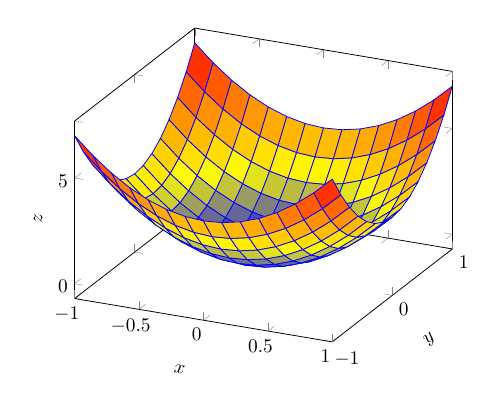
\begin{tikzpicture}[scale=\scale]
		\begin{axis}[
			xlabel=$x$,
			ylabel=$y$,
			zlabel=$z$,
			xlabel style={sloped},
			ylabel style={sloped},
		]
			\addplot3[
				surf,
				faceted color=blue,
				samples=15,
				domain=-1:1,y domain=-1:1
			]{3*x^2+4*y^2};
		\end{axis}
	\end{tikzpicture}~\begin{tikzpicture}[scale=\scale]
		\begin{axis}[
			xlabel=$x$,
			ylabel=$z$,
		]
			\addplot[
				surf,
				faceted color=blue,
				samples=30,
				domain=-1:1
			]{3*x^2};
		\end{axis}
	\end{tikzpicture}
	\caption{}%@see:[example:多元函数的极值.例1]
	\label{figure:多元函数的极值.例1}
\end{figure}

\subsection{多元函数极值存在的条件}
二元函数的极值问题,一般可以利用偏导数来解决.
下面两个定理就是关于这个问题的结论.
\begin{theorem}[必要条件]\label{theorem:多元函数微分法.多元函数极值存在的必要条件}
设函数\(z=f(x,y)\)在点\(P_0(x_0,y_0)\)具有偏导数,且在点\(P_0\)处有极值,则有\[
	f'_x(x_0,y_0) = f'_y(x_0,y_0) = 0.
\]
\begin{proof}
不妨设\(z=f(x,y)\)在点\((x_0,y_0)\)处有极大值.
根据定义,
在点\((x_0,y_0)\)的某去心邻域内的点\((x,y)\)都满足不等式\[
	f(x,y)<f(x_0,y_0).
\]
特别地,在该邻域内取\(y=y_0\)而\(x\neq x_0\)的点,也应满足不等式\[
	f(x,y_0)<f(x_0,y_0).
\]
这表明一元函数\(f(x,y_0)\)在\(x=x_0\)处取得极大值,
因而必有\[
	f'_x(x_0,y_0)=0.
\]

类似地可证\[
	f'_y(x_0,y_0)=0.
\]
\end{proof}
\end{theorem}

从几何上看,这时如果曲面\(z=f(x,y)\)在点\((x_0,y_0,z_0)\ (z_0=f(x_0,y_0))\)处有切平面,
则切平面\[
	z-z_0=f'_x(x_0,y_0)(x-x_0)+f'_y(x_0,y_0)(y-y_0)
\]成为平行于\(xOy\)坐标面的平面\(z=z_0\).

仿照一元函数,我们给出多元函数的“驻点”的定义.
\begin{definition}
设函数\(f\colon D \to \mathbb{R}\),\(D \subseteq \mathbb{R}^n\),
\(P_0\)为\(D\)的内点.
若\[
	\pdv{f}{x_i}\eval_{P_0}=0
	\quad(i=1,2,\dotsc,n),
\]
则称“点\(P_0\)称为函数\(f\)的\DefineConcept{驻点}”.
\end{definition}
那么\cref{theorem:多元函数微分法.多元函数极值存在的必要条件}
可以说成“具有偏导数的函数的极值点必定是驻点,但函数的驻点不一定是极值点”.
例如,点\((0,0)\)是函数\(f(x,y) = xy\)的驻点,但函数\(f\)在该点并无极值.

\begin{theorem}[充分条件]\label{theorem:多元函数微分法.多元函数极值存在的充分条件}
设函数\(z=f(x,y)\)在点\(P_0(x_0,y_0)\)的某一邻域内连续且有一阶及二阶连续偏导数,
又\(f'_x(x_0,y_0)=0\),\(f'_y(x_0,y_0)=0\),
令\[
	f''_{xx}(x_0,y_0)=A, \quad
	f''_{xy}(x_0,y_0)=B, \quad
	f''_{yy}(x_0,y_0)=C,
\]
则\(f(x,y)\)在\((x_0,y_0)\)处是否取得极值的条件如下:
\begin{enumerate}
	\item \(AC-B^2>0\)时具有极值,且当\(A<0\)时有极大值,当\(A>0\)时有极小值;
	\item \(AC-B^2<0\)时没有极值;
	\item \(AC-B^2=0\)时可能有极值,也可能没有极值.
\end{enumerate}
\end{theorem}

\begin{example}
当\(AC-B^2=0\)时,函数可能有极值,也可能没有极值;
即便函数有极值,可能是极大值,也可能是极小值.
对于以下三个函数\[
	f(x,y) = x^2 y^2,
	\qquad
	g(x,y) = -x^2 y^2,
	\qquad
	h(x,y) = x^2 y^3,
\]
它们在原点\((0,0)\)处都有\(AC-B^2=0\),
但是\(f\)在原点取极小值,\(g\)在原点取极大值,而\(h\)在原点没有极值.
\end{example}

\begin{example}
求函数\(f(x,y) = x^3-y^3+3x^2+3y^2-9x\)的极值.
\begin{solution}
先解方程组\[
	\left\{ \begin{array}{l}
		f'_x(x,y) = 3x^2+6x-9 = 0, \\
		f'_y(x,y) = -3y^2+6y = 0,
	\end{array} \right.
\]
求得驻点为\(\opair{1,0},\opair{1,2},\opair{-3,0},\opair{-3,2}\).

再求出二阶偏导数\[
	f''_{xx}(x,y) = 6x+6,
	\qquad
	f''_{xy}(x,y) = 0,
	\qquad
	f''_{yy}(x,y) = -6y+6.
\]

在点\(\opair{1,0}\)处,\(AC-B^2=12\cdot6>0\),又\(A=12>0\),
所以函数在\(\opair{1,0}\)处有极小值\(f(1,0)=-5\);
在点\(\opair{1,2}\)处,\(AC-B^2=12\cdot(-6)<0\),
所以点\(\opair{1,2}\)不是极值点;
在点\(\opair{-3,0}\)处,\(AC-B^2=(-12)\cdot6<0\),
所以点\(\opair{-3,0}\)不是极值点;
在点\(\opair{-3,2}\)处,\(AC-B^2=(-12)\cdot(-6)>0\),又\(A=-12<0\),
所以函数在\(\opair{-3,2}\)处有极大值\(f(-3,2)=31\).
\end{solution}
\end{example}

\begin{example}
求函数\(f(x,y) = (y-x^2)(y-x^3)\)的极值.
\begin{solution}
对\(f(x,y) = y^2 - (x^2+x^3) y + x^5\)求偏导,得\[
f'_x = 5x^4 - y(2x+3x^2),
\qquad
f'_y = 2y - x^2 - x^3.
\]

令\(f'_x = f'_y = 0\).
当\(x=0\)时,解得\(y = 0\);
当\(x\neq0\)时,有\[
\begin{cases}
5x^4-y(2x+3x^2) = 0, \\
2y-x^2+x^3 = 0,
\end{cases}
\]于是\[
5x^4 = \frac{x^2+x^3}{2}(2x+3x^2),
\]整理得\[
3x^5-5x^4+2x^3=0,
\]即\[
3x^2-5x+2=0,
\]解得\(x=1,y=1\)或\(x=2/3,y=10/27\).
也就是说,函数\(f\)的驻点为\[
(0,0), \qquad
\opair{1,1}, \qquad
\opair{2/3,10/27}.
\]

再对\(f\)求二阶偏导,得\[
f''_{xx} = 20x^3 - y(2+6x),
\qquad
f''_{xy} = -2x-3x^2,
\qquad
f''_{yy} = 2.
\]
那么
\[
f''_{xx}(0,0) = 0,
\qquad
f''_{xy}(0,0) = 0,
\qquad
f''_{yy}(0,0) = 2,
\]\[
f''_{xx}(1,1) = 12,
\qquad
f''_{xy}(1,1) = -5,
\qquad
f''_{yy}(1,1) = 2,
\]\[
f''_{xx}(2/3,10/27) = 100/27,
\qquad
f''_{xy}(2/3,10/27) = -8/3,
\qquad
f''_{yy}(2/3,10/27) = 2.
\]

在点\((0,0)\)处\(AC-B^2 = 0\);
取\(k>0\),由于\[
f(-k,0) = -k^5 < f(0,0) = 0 < f(k,0) = k^5,
\]所以函数\(f\)在点\((0,0)\)处不存在极值.

在点\(\opair{1,1}\)处\(AC-B^2 < 0\),
所以函数\(f\)在点\(\opair{1,1}\)处也没有极值.

在点\(\opair{2/3,10/27}\)处\(AC-B^2 > 0\)且\(A>0\),
所以函数\(f\)在点\(\opair{2/3,10/27}\)处存在极小值\[
f(2/3,10/27) = -4/729.
\]
\end{solution}
\end{example}

我们进一步推广到\(n\)元函数上.
\begingroup
\def\x{\mat{X}}
\def\X#1{\x_{#1}}
\def\z{\mat{0}}

\begin{theorem}\label{theorem:多元函数微分法.n元函数极值存在的条件}
设函数\(y = f(\AutoTuple{x}{n})\)在点\(\X0=(\AutoTuple{\xi}{n})^T\in\mathbb{R}^n\)的邻域内%
存在一阶连续偏导数\[
	f'_i = \pdv{f}{x_i}
	\quad(i=1,2,\dotsc,n)
\]
和二阶连续偏导数\[
	f''_{ij} = \pdv[2]{f}{x_i}{x_j}
	\quad(i,j=1,2,\dotsc,n).
\]
记\(f\)的梯度为\(\grad f(\x) = \left(\pdv{f}{x_1},\pdv{f}{x_2},\dotsc,\pdv{f}{x_n}\right)^T\),
\(f\)的黑森矩阵为\(\hessian f = (f''_{ij})_n\),
则\begin{enumerate}
\item 当\(\grad f(\X0) = \z\),且\(\hessian f\)正定时,\(f(\x)\)在\(\X0\)处取得极小值;
\item 当\(\grad f(\X0) = \z\),且\(\hessian f\)负定时,\(f(\x)\)在\(\X0\)处取得极大值;
\item 当\(\grad f(\X0) = \z\),且\(\hessian f\)半正定或半负定时,\(f(\x)\)可能有极值,也可能没有极值\footnote{%
这时候需要考察更高阶偏导数,才能确定函数的极值是否存在,是极大值还是极小值.%
};
\item 当\(\grad f(\X0) = \z\),且\(\hessian f\)不定时,\(\X0\)不是\(f(\x)\)的极值点.
\end{enumerate}
\begin{proof}
将\(y = f(\x)\)在\(\X0\)处作泰勒展开,得\[
f(\x) = f(\X0)
+ \sum\limits_{i=1}^n f'_i(\X0) h_i
+ \frac{1}{2} \sum\limits_{i=1}^n \sum\limits_{j=1}^n
	f''_{ij}(\X0+\theta\increment\x) h_i h_j,
\]其中\(\increment\x=\x-\X0=(h_1,h_2,\dotsc,h_n)^T,%
h_i = x_i - x_{i0}\ (i=1,2,\dotsc,n),%
0<\theta<1\).

由于\(\grad f(\X0) = \z\)且\(f(\x)\)的所有二阶偏导数连续,故\(\sum\limits_{i=1}^n f'_i(\X0) h_i = 0\),\begin{align*}
f(\x) - f(\X0)
&= \frac{1}{2} \sum\limits_{i=1}^n \sum\limits_{j=1}^n
	f''_{ij}(\X0+\theta\increment\x) h_i h_j \\
&= \frac{1}{2} \sum\limits_{i=1}^n \sum\limits_{j=1}^n
	f''_{ij}(\X0) h_i h_j
	+ \frac{1}{2} \sum\limits_{i=1}^n \sum\limits_{j=1}^n
	\varepsilon_{ij} h_i h_j \\
&= \frac{1}{2} (\increment\x)^T [\hessian f + (\varepsilon_{ij})_n] (\increment\x),
\end{align*}
其中\(\varepsilon_{ij} = f''_{ij}(\X0+\theta\increment\x) - f''_{ij}(\X0)\),且\[
\varepsilon_{ij} = \varepsilon_{ji}\to0\ (\increment\x\to\z)
\quad(i,j=1,2,\dotsc,n).
\]

当实对称矩阵\(\hessian f\)正定时,其各阶顺序主子式全大于零,
那么根据行列式的定义和极限的保号性,当\(\abs{\increment\x}\to0\)时,
\(\hessian f + (\varepsilon_{ij})_n\)的各阶顺序主子式也全大于零,
故\(\hessian f + (\varepsilon_{ij})_n\)依然正定,便得\(f(\x) - f(\X0) > 0\),
也就是说\(f(\x)\)在\(\X0\)取到极大值\(f(\X0)\).

同理可证其他两种情形下的结论.
\end{proof}
\end{theorem}

\begin{example}
求函数\(f(x,y) = 2x^2 + xy + y^2 + ax - 5y\)的极值.
\begin{solution}
显然,函数\(f\)的各阶偏导数都连续.
令\[
\grad f(x,y) = \begin{bmatrix} f'_x \\ f'_y \end{bmatrix}
= \begin{bmatrix} 4x+y+a \\ x+2y-5 \end{bmatrix} = \z,
\]解得驻点为\(\X0 = \frac{1}{7} \begin{bmatrix} -5-2a \\ 20+a \end{bmatrix}\).
\(\hessian f = \begin{bmatrix}
f''_{11} & f''_{12} \\
f''_{21} & f''_{22}
\end{bmatrix} = \begin{bmatrix}
4 & 1 \\
1 & 2
\end{bmatrix}\)是正定矩阵,故\(f\)在\(\X0\)处取得极小值\(\frac{1}{7} (-50-5a-a^2)\).
\end{solution}
\end{example}

\subsection{极值点的求解思路}
利用\cref{theorem:多元函数微分法.多元函数极值存在的必要条件,%
theorem:多元函数微分法.多元函数极值存在的充分条件,%
theorem:多元函数微分法.n元函数极值存在的条件},
我们把具有二阶连续偏导数的函数\(z = f(x,y)\)的极值的求法叙述如下:
\begin{enumerate}
	\item 解方程组\[
		f'_x(x,y) = 0
		\quad\text{和}\quad
		f'_y(x,y) = 0,
	\]求得一切实数解,即可求得一切驻点.

	\item 对于每一个驻点\((x_0,y_0)\),
	求出二阶偏导数的值\(A=f''_{xx}\)、\(B=f''_{xy}\)和\(C=f''_{yy}\).

	\item 定出\(AC-B^2\)的符号,
	按\cref{theorem:多元函数微分法.多元函数极值存在的充分条件}
	的结论判定\(f(x_0,y_0)\)是不是极值,是极大值还是极小值.
	当\(AC-B^2=0\)时,可以借助极值的定义判断是否存在极值以及极值的类型.
\end{enumerate}

讨论函数的极值问题时,如果函数在所讨论的区域内具有偏导数,则极值只可能在驻点处取得.
然而,如果函数在个别点处的偏导数不存在,这些点当然不是驻点,但也可能是极值点.
例如,函数\(f(x,y) = -\sqrt{x^2+y^2}\)在点\((0,0)\)处的偏导数不存在,
但该函数在点\((0,0)\)处却具有极大值.
因此,在考虑函数的极值问题时,除了考虑函数的驻点外,
如果有偏导数不存在的点,那么对这些点也应当考虑.

\subsection{最值点的求解思路}
与一元函数相类似,我们可以利用函数的极值来求函数的最值.
我们知道,如果\(f(x,y)\)在有界闭区域\(D\)上连续,
则\(f(x,y)\)在\(D\)上必定能取得最大值和最小值.
这种使函数取得最大值或最小值的点(即最值点)既可能在\(D\)的内部,也可能在\(D\)的边界上.
我们假定,函数在\(D\)上连续,在\(D\)内可微分且只有有限个驻点,
这时如果函数在\(D\)的内部取得最大值(或最小值),则这个最值也是函数的极值.
因此,这上述假定下,求函数的最值的一般方法是:
将函数\(f(x,y)\)在\(D\)内的所有驻点处的函数值及在\(D\)的边界上的最值相互比较,
其中最大的就是最大值,最小的就是最小值.
但这种做法,由于要求出\(f(x,y)\)在\(D\)的边界上的最值,所以往往相当复杂.
在通常遇到的实际问题中,如果根据问题的性质,
知道函数\(f(x,y)\)的最值一定在\(D\)的内部取得,
而函数在\(D\)内只有一个驻点,
那么可以肯定该驻点处的函数值就是函数\(f(x,y)\)在\(D\)上的最值.

\subsection{拉格朗日乘数法 --- 条件极值的求解思路}\label{subsection:多元函数微分法.拉格朗日乘数法}
上面所讨论的极值问题,对于函数的自变量,除了限制在函数的定义域内以外,
并无其他条件,所以有时候称为\DefineConcept{无条件极值}.
但在实际问题中,有时会遇到对函数的自变量还有附加条件的极值问题.
例如,求表面积为\(a^2\)而体积为最大的长方体的体积问题.
设长方体的三棱的长为\(x,y,z\),则体积为\(V = xyz\).
又因假定表面积为\(a^2\),所以自变量\(x,y,z\)还必须满足附加条件\(2(xy+yz+zx)=a^2\).
像这种对自变量有附加条件的极值称为\DefineConcept{条件极值}.
对于有些实际问题,可以把条件极值化为无条件极值,然后利用前面的方法加以解决.
例如上述问题,可由条件\(2(xy+yz+zx)=a^2\),将\(z\)表成\(x,y\)的函数\[
	z = \frac{a^2-2xy}{2(x+y)}.
\]
再把它代入\(V = xyz\)中,于是问题就化为求\[
	V = \frac{xy}{2} \frac{a^2-2xy}{x+y}
\]的无条件极值.

但在很多情形下,将条件极值化为无条件极值并不这样简单.
另有一种直接寻求条件极值的方法,可以不必先把问题化到无条件极值的问题,
这就是下面要介绍的\DefineConcept{拉格朗日乘数法}.

我们先寻求函数
\begin{equation}\label{equation:拉格朗日乘数法.目标函数1}
%@see: 《高等数学(第六版 下册)》 P114. 公式(1)
	z=f(x,y)
\end{equation}
在条件
\begin{equation}\label{equation:拉格朗日乘数法.限制条件1}
%@see: 《高等数学(第六版 下册)》 P114. 公式(2)
	\varphi(x,y)=0
\end{equation}
下取得极值的必要条件.

如果函数 \labelcref{equation:拉格朗日乘数法.目标函数1}
在\(P_0(x_0,y_0)\)取得所求的极值,
那么首先有
\begin{equation}\label{equation:拉格朗日乘数法.限制条件1在P0}
%@see: 《高等数学(第六版 下册)》 P114. 公式(3)
	\varphi(x_0,y_0)=0.
\end{equation}
我们假定在\((x_0,y_0)\)的某一邻域内
\(f(x,y)\)与\(\varphi(x,y)\)均有连续的一阶偏导数,
而\(\varphi'_y(x_0,y_0)\neq0\).
由隐函数存在定理可知,
方程 \labelcref{equation:拉格朗日乘数法.限制条件1}
确定一个连续且具有连续导数的函数\(y=\psi(x)\),
将其代入\cref{equation:拉格朗日乘数法.目标函数1},
结果得到一个变量\(x\)的函数
\begin{equation}\label{equation:拉格朗日乘数法.目标函数1.代入限制条件1}
%@see: 《高等数学(第六版 下册)》 P114. 公式(4)
	z=f(x,\psi(x)).
\end{equation}
于是函数 \labelcref{equation:拉格朗日乘数法.目标函数1} 在\((x_0,y_0)\)取得所求的极值,
也就是相当于函数 \labelcref{equation:拉格朗日乘数法.目标函数1.代入限制条件1} 在\(x=x_0\)取得极值.
由一元可导函数取得极值的必要条件知道
\begin{equation}\label{equation:拉格朗日乘数法.目标函数1取得极值的必要条件1}
%@see: 《高等数学(第六版 下册)》 P114. 公式(5)
	\dv{z}{x}\eval_{x=x_0}
	= f'_x(x_0,y_0) + f'_y(x_0,y_0) \dv{y}{x}\eval_{x=x_0}
	= 0,
\end{equation}
而由\cref{equation:拉格朗日乘数法.限制条件1} 用隐函数求导公式,有\[
	\dv{y}{x}\eval_{x=x_0}
	= -\frac{\varphi'_x(x_0,y_0)}{\varphi'_y(x_0,y_0)}.
\]
把上式代入\cref{equation:拉格朗日乘数法.目标函数1取得极值的必要条件1},得
\begin{equation}\label{equation:拉格朗日乘数法.目标函数1取得极值的必要条件2}
%@see: 《高等数学(第六版 下册)》 P114. 公式(6)
	f'_x(x_0,y_0) - f'_y(x_0,y_0) \frac{\varphi'_x(x_0,y_0)}{\varphi'_y(x_0,y_0)}
	= 0.
\end{equation}
\labelcref{equation:拉格朗日乘数法.限制条件1在P0,equation:拉格朗日乘数法.目标函数1取得极值的必要条件2}
两式就是函数 \labelcref{equation:拉格朗日乘数法.目标函数1}
在条件 \labelcref{equation:拉格朗日乘数法.限制条件1} 下
在\((x_0,y_0)\)取得极值的必要条件.

令\(\lambda=-\frac{f'_y(x_0,y_0)}{\varphi'_y(x_0,y_0)}\),
则上述必要条件就变为
\begin{equation}\label{equation:拉格朗日乘数法.目标函数1取得极值的必要条件3}
	\left\{ \begin{array}{l}
		f'_x(x_0,y_0) + \lambda \varphi'_x(x_0,y_0) = 0, \\
		f'_y(x_0,y_0) + \lambda \varphi'_y(x_0,y_0) = 0, \\
		\varphi(x_0,y_0) = 0.
	\end{array} \right.
\end{equation}

若引进辅助函数\[
	L(x,y) = f(x,y) + \lambda \varphi(x,y),
\]
则不难看出,
\cref{equation:拉格朗日乘数法.目标函数1取得极值的必要条件3} 中前两式就是\[
	L'_x(x_0,y_0)=0, \qquad
	L'_y(x_0,y_0)=0.
\]
我们把函数\(L(x,y)\)称为\DefineConcept{拉格朗日函数},
把参数\(\lambda\)称为\DefineConcept{拉格朗日乘子}.

由以上讨论,我们得到以下结论.

要找函数\(z=f(x,y)\)在附加条件\(\varphi(x,y)=0\)下的可能极值点,
可以先作拉格朗日函数\[
	L(x,y) = f(x,y) + \lambda \varphi(x,y),
\]
其中\(\lambda\)为参数.
求其对\(x\)与\(y\)的一阶偏导数,并使之为零,
然后与限定条件方程联立起来:\[
	\left\{ \begin{array}{l}
		f'_x(x,y)+\lambda\varphi'_x(x,y)=0, \\
		f'_y(x,y)+\lambda\varphi'_y(x,y)=0, \\
		\varphi(x,y)=0.
	\end{array} \right.
\]
由这方程组解出\(x,y,\lambda\),
这样得到的\(\opair{x,y}\)就是函数\(f(x,y)\)在附件条件\(\varphi(x,y)=0\)下的可能极值点.

这方法还可以推广到自变量多于两个而条件多于一个的情形.
例如,要求函数\[
	f\colon \mathbb{R}^n \to \mathbb{R}, P = (\AutoTuple{x}{n})^T \mapsto u
\]在\(m\ (m<n)\)个附加条件\[
	\varphi_i(P) = 0
	\quad(i=1,2,\dotsc,m)
\]下的极值,
可以先作拉格朗日函数\[
	L(P) = f(P) + \sum_{i=1}^m \lambda_i \varphi_i(P),
\]
其中\(\lambda_k\ (k=1,2,\dotsc,m)\)均为参数.
求其一阶偏导数,并使之为零,然后与条件方程组联立起来求解,即\[
	\left\{ \def\arraystretch{1.5} \begin{array}{ll}
		\pdv{L}{x_i}\eval_P = 0 & (i=1,2,\dotsc,n), \\
		\varphi_j(P) = 0 & (j=1,2,\dotsc,m).
	\end{array} \right.
\]
这样得出的点\(P\)就是函数\(f(P)\)在附加条件方程组下的可能极值点.

至于如何确定所求得的点是否极值点,在实际问题中往往可根据问题本身的性质来判定.

\begin{example}
求表面积为\(a^2\)而体积为最大的长方体的体积.
\begin{solution}
设长方体的三棱长为\(x,y,z\),
则问题就是在条件\[
	\varphi(x,y,z) = 2xy+2yz+2zx-a^2 = 0
	\eqno(1)
\]下,
求函数\[
	V = xyz
	\quad (x>0,y>0,z>0)
	\eqno(2)
\]的最大值.
作拉格朗日函数\[
	L(x,y,z) = xyz + \lambda(2xy+2yz+2zx-a^2),
\]
求其对\(x,y,z\)的偏导数,并使之为零,得到\[
	\left\{ \begin{array}{l}
		yz+2\lambda(y+z) = 0, \\
		xz+2\lambda(x+z) = 0, \\
		xy+2\lambda(y+x) = 0.
	\end{array} \right.
	\eqno(3)
\]
因\(x,y,z\)都不等于零,所以由(3)式可得\[
	\frac{x}{y} = \frac{x+z}{y+z},
	\qquad
	\frac{y}{z} = \frac{x+y}{x+z}.
\]
由以上两式解得\[
x=y=z.
\]
将此代入(1)式,得\[
	x = y = z = \frac{\sqrt{6}}{6} a,
\]
这是唯一可能的极值点.
因为由问题本身可知最大值一定存在,所以最大值就在这个可能的极值点处取得.
也就是说,表面积为\(a^2\)的长方体中,
以棱长为\(\frac{\sqrt{6}}{6}a\)的正方体的体积为最大,
最大体积\(V = \frac{\sqrt{6}}{36} a^3\).
\end{solution}
\end{example}

\begin{example}
求函数\(u=xyz\)在附加条件\[
	\frac{1}{x}+\frac{1}{y}+\frac{1}{z}=\frac{1}{a}
	\quad(x>0,y>0,z>0,a>0)
\]下的极值.
\begin{solution}
作拉格朗日函数\[
	L(x,y,z) = xyz+\lambda\left(\frac{1}{x}+\frac{1}{y}+\frac{1}{z}-\frac{1}{a}\right).
\]
令\[
	L'_x = yz - \frac{\lambda}{x^2} = 0,
	\qquad
	L'_y = xz - \frac{\lambda}{y^2} = 0,
	\qquad
	L'_z = xy - \frac{\lambda}{z^2} = 0.
\]
注意到以上三个方程左端的第一项都是三个变量\(x,y,z\)中某两个变量的乘积,
将各方程两端同乘以相应缺少的那个变量,使得各方程左端的第一项都成为\(xyz\),
然后将所得的三个方程左、右两端相加,得\[
	3xyz - \lambda\left(\frac{1}{x}+\frac{1}{y}+\frac{1}{z}\right) = 0,
\]
代入附加条件,得\[
	xyz = \frac{\lambda}{3a}.
\]
再把这个结果分别代入偏微分方程组,便得\(x = y = z = 3a\).
由此得到点\(\opair{3a,3a,3a}\)是函数\(u = xyz\)在给定的附加条件下唯一可能的极值点.

把附加条件确定的隐函数记作\(v = z(x,y)\),将目标函数看作\(u = xyv = F(x,y)\),\[
\pdv{F}{x} = y\left(v+x\pdv{v}{x}\right);
\]再运用\cref{theorem:多元函数微分法.多元函数极值存在的充分条件} 判断,
可知点\(\opair{3a,3a,3a}\)是函数\(u = xyz\)在给定附加条件下的极小值点,
函数\(u = xyz\)在该点处取得极小值\(27a^3\).
\end{solution}
\end{example}

\section{最小二乘法}
许多科学、工程问题常常需要根据两个或者多个变量的几次实验数据
来找出这些变量的(近似)关系式(称这些依据实验数据建立的近似关系式为经验公式).
在建立经验公式的过程中,经常使用线性数学模型拟合实验数据.
但是在测量时因为受到了各种条件的限制,我们往往得到的是一个不相容(无解)的线性方程组,
不过我们可以采用“最小二乘法”求出线性方程组的近似解.

我们首先考虑只有两个变量(一个作为自变量,一个作为因变量)的情形.

已知点列\(\{P_n\}\).
假设点列中的所有点\(\opair{x_k,y_k}\ (k=1,2,\dotsc,n)\)都近似满足直线方程\[
	f(x) = a x + b,
\]
再根据偏差的平方和\[
	M(a,b) = \sum\limits_k [y_k - f(x_k)]^2 = \sum\limits_k [y_k - (a x_k + b)]^2
\]为最小的条件来选择常数\(a,b\).

令\[
	\left\{ \begin{array}{l}
		\pdv{M}{a} = -2 \sum\limits_k [y_k - (a x_k + b)] x_k = 0, \\
		\pdv{M}{b} = -2 \sum\limits_k [y_k - (a x_k + b)] = 0,
	\end{array} \right.
\]
那么有\[
	\left\{ \begin{array}{l}
		\sum\limits_k x_k y_k = a \sum\limits_k x_k^2 + b \sum\limits_n x_k, \\
		\sum\limits_k y_k = a \sum\limits_k x_k + b n. \\
	\end{array} \right.
\]
现在只要首先将\[
	\sum\limits_k x_k, \qquad
	\sum\limits_k x_k^2, \qquad
	\sum\limits_k x_k y_k, \qquad
	\sum\limits_k y_k
\]计算出来,代入以上代数方程组,即可解出合适的\(a\)和\(b\)使得\(M(a,b)\)取得最小值.

现在我们将上面的方法推广到有\(n\)个自变量和\(s\)个因变量的情形.

\def\A{\mat{A}}
\def\b{\mat{\beta}}
设\(\A = (a_{ij})_{s \times n} \in M_{s \times n}(\mathbb{R})\),
\(\b = (b_1,b_2,\dotsc,b_s)^T \in \mathbb{R}^s\),
\(\x = (\AutoTuple{x}{n})^T\),
线性方程组\(\A\x=\b\)无解(即\(\rank(\A,\b)>\rank\A\)).
那么\[
	f(\x) = \abs{\A\x=\b}^2
	= \sum\limits_{i=1}^s (a_{i1} x_1 + a_{i2} x_2 + \dotsb + a_{in} x_n - b_i)^2
	> 0.
\]
现在我们想要找到能使\(f(\x)\)取得最小值的\(\X0\),称这个\(\X0\)的\DefineConcept{最小二乘解}.

\endgroup
